% ******************************************************************	********************************************
%
% **************************************************************************************************************
\documentclass[ twoside,openright,titlepage,numbers=noenddot,%
								toc=bibliography,toc=listof,%
                footinclude=false,headinclude=false,cleardoublepage=empty,%
								BCOR=5mm,paper=a4,fontsize=11pt,%DIV=14,%
                ngerman%
                ]{scrreprt}

%***************************************************************************************************************
% Note: Make all your adjustments in here
%***************************************************************************************************************
% ****************************************************************************************************
% htwsaar-i-mst-config.tex 
% ****************************************************************************************************  
\RequirePackage[utf8]{inputenc}				
 \DeclareUnicodeCharacter{00A0}{~}								
\RequirePackage[T1]{fontenc} 
								
% ****************************************************************************************************
% 1. Personal data and user ad-hoc commands
% ****************************************************************************************************
\newcommand{\myTitle}{Implementierung elliptischer Kurven für die Kryptographie}
\newcommand{\myDegree}{Projektarbeit\xspace}
%\newcommand{\myDegree}{Master of Science (M.\,Sc.)\xspace}
\newcommand{\myDegreeType}{Projektbericht\xspace}
%\newcommand{\myDegreeType}{Master\xspace}
\newcommand{\myDegreeCourse}{Praktische Informatik}
%\newcommand{\myDegreeCourse}{Kommunikationsinformatik}
\newcommand{\myName}{Annick Aboa\xspace}
\newcommand{\mysecondName}{Hendrik Haas\xspace}
\newcommand{\mythirdName}{Mai Manh-Khang\xspace}
\newcommand{\myUni}{Hochschule für Technik und Wirtschaft des Saarlandes\xspace}
\newcommand{\myCompany}{SoftwareCenter Musterhausen\xspace}
\newcommand{\myFirstProf}{Prof. Dr. Peter Birkner\xspace}
\newcommand{\mySecondProf}{Prof. Dr. Thomas Kretschmer\xspace}
\newcommand{\myLocation}{Saarbrücken\xspace}
\newcommand{\myTime}{31.~März~2021\xspace}
\newcommand{\currentVersion}{Version 2.1\xspace} % TODO: ggf. über git Versionsinformationen automatisch bereitstellen und verwenden

% ********************************************************************
% Setup, finetuning, and useful commands
% ********************************************************************
\newcounter{dummy} % necessary for correct hyperlinks (to index, bib, etc.)
% ****************************************************************************************************


% ****************************************************************************************************
% 2. Loading some handy packages
% ****************************************************************************************************
% ******************************************************************** 
% Packages with options that might require adjustments
% ******************************************************************** 
\PassOptionsToPackage{ngerman}{babel}   % change this to your language(s)
 \RequirePackage{babel}					
 \RequirePackage{csquotes}
	
\PassOptionsToPackage{language=auto,style=numeric-comp,backend=bibtex8,bibencoding=ascii,maxbibnames=50}{biblatex}
 \RequirePackage{biblatex}	
 \bibliography{Bibliography}			

\PassOptionsToPackage{fleqn}{amsmath}		% math environments and more by the AMS 
 \RequirePackage{amsmath}

% ******************************************************************** 
% Setting up the page and margins
% ******************************************************************** 
\usepackage{geometry}
 \geometry{a4paper,left=25mm,right=35mm,top=25mm,bottom=30mm}
% DIESE WERTE SIND NICHT ZU VERÄNDERN -- DO NOT CHANGE THESE VALUES

% ******************************************************************** 
% General useful packages
% ******************************************************************** 
%\usepackage[automark]{scrpage2}
\PassOptionsToPackage{dvipsnames}{xcolor}
	\RequirePackage{xcolor} % [dvipsnames]  
	\definecolor{ingwi}{cmyk}{.9,0,0,0}
\usepackage{textcomp} % fix warning with missing font shapes
\usepackage{scrhack} % fix warnings when using KOMA with listings package          
\usepackage{xspace} % to get the spacing after macros right  
\usepackage{mparhack} % get marginpar right
%\usepackage{fixltx2e} % fixes some LaTeX stuff <-- ist seit 2015 nicht mehr notwendig
\PassOptionsToPackage{printonlyused}{acronym}
	\usepackage{acronym} % nice macros for handling all acronyms in the thesis
%\renewcommand{\bflabel}[1]{{#1}\hfill} % fix the list of acronyms
\usepackage{booktabs}
\usepackage{polynom}
\usepackage{multirow}
\usepackage[shadow]{todonotes} %Settings for ToDoNotes
% Eigene Shortcuts fuer laengere Befehle
	\newcommand{\todox}[1]{\todo[inline, size=\small]{#1}}
	%Nummerierte Anmerkungen
	\newcounter{todocounter}
	\renewcommand{\todox}[2][]{\stepcounter{todocounter}\todo[inline, size=\small,caption={\thetodocounter: #2}, #1]{\renewcommand{\baselinestretch}{0.5}\selectfont\thetodocounter: #2\par}}
\usepackage{blindtext}
%\usepackage{footmisc}
% ****************************************************************************************************


% ****************************************************************************************************
% 3. Setup floats: tables, (sub)figures, and captions
% ****************************************************************************************************
\usepackage{tabularx} % better tables
	\setlength{\extrarowheight}{3pt} % increase table row height
%\newcommand{\myfloatalign}{\centering} % to be used with each float for alignment
\usepackage{caption}
\captionsetup{format=hang,font=small}
\usepackage{subfig}
\usepackage{wrapfig}
% ****************************************************************************************************


% ****************************************************************************************************
% 6. Setup code listings
% ****************************************************************************************************
\usepackage{listings} 
%\lstset{emph={trueIndex,root},emphstyle=\color{BlueViolet}}%\underbar} % for special keywords
\lstset{language=[LaTeX]Tex,%C++,
    keywordstyle=\color{RoyalBlue},%\bfseries,
    basicstyle=\small\ttfamily,
    %identifierstyle=\color{NavyBlue},
    commentstyle=\color{Green}\ttfamily,
    stringstyle=\rmfamily,
    numbers=none,%left,%
    numberstyle=\scriptsize,%\tiny
    stepnumber=5,
    numbersep=8pt,
    showstringspaces=false,
    breaklines=true,
    frameround=ftff,
    frame=single,
		texcl=true,
    belowcaptionskip=.75\baselineskip
    %frame=L
} 
%Styles für verschiedene Sprachen festlegen, z.B. Java
\lstdefinestyle{Java}{
belowcaptionskip=1\baselineskip,
  breaklines=true,
  xleftmargin=\parindent,
  language=Java,
	texcl=true,
  showstringspaces=false,
  basicstyle=\footnotesize\ttfamily,
  keywordstyle=\bfseries\color{green!40!black},
  commentstyle=\itshape\color{purple!40!black},
  identifierstyle=\color{blue},
  stringstyle=\color{orange}}
% ****************************************************************************************************    		   


% ****************************************************************************************************
% 6. PDFLaTeX, hyperreferences and citation backreferences
% ****************************************************************************************************
% ********************************************************************
% Using PDFLaTeX
% ********************************************************************
\PassOptionsToPackage{pdftex,hyperfootnotes=false,pdfpagelabels}{hyperref}
	\usepackage{hyperref}  % backref linktocpage pagebackref
\pdfcompresslevel=9
\pdfadjustspacing=1 
\PassOptionsToPackage{pdftex}{graphicx}
	\usepackage{graphicx} 
    

% ********************************************************************
% Hyperreferences
% ********************************************************************
\hypersetup{%
    %draft,	% = no hyperlinking at all (useful in b/w printouts)
    pdfstartpage=1, pdfstartview=Fit,%
		colorlinks=true, linktocpage=true,
		%urlcolor=Black, linkcolor=Black, citecolor=Black, %pagecolor=Black,%
		%urlcolor=brown, linkcolor=RoyalBlue, citecolor=green, %pagecolor=RoyalBlue,%
    % uncomment the following line if you want to have black links (e.g., for printing)
    colorlinks=false, pdfborder={0 0 0},
    breaklinks=true, pdfpagemode=UseNone, pageanchor=true, pdfpagemode=UseOutlines,%
    plainpages=false, bookmarksnumbered, bookmarksopen=true, bookmarksopenlevel=1,%
    hypertexnames=true, pdfhighlight=/O,%nesting=true,%frenchlinks,%
    pdftitle={\myTitle},%
    pdfauthor={\textcopyright\ \myName, \myUni},%
    pdfsubject={},%
    pdfkeywords={},%
    pdfcreator={pdfLaTeX},%
    pdfproducer={LaTeX with hyperref}%
}   

% ********************************************************************
% Setup autoreferences
% ********************************************************************
% There are some issues regarding autorefnames
% http://www.ureader.de/msg/136221647.aspx
% http://www.tex.ac.uk/cgi-bin/texfaq2html?label=latexwords
% you have to redefine the makros for the 
% language you use, e.g., american, ngerman
% (as chosen when loading babel/AtBeginDocument)
% ********************************************************************
\makeatletter
\@ifpackageloaded{babel}%
    {%
       \addto\extrasamerican{%
					\renewcommand*{\figureautorefname}{Figure}%
					\renewcommand*{\tableautorefname}{Table}%
					\renewcommand*{\partautorefname}{Part}%
					\renewcommand*{\chapterautorefname}{Chapter}%
					\renewcommand*{\sectionautorefname}{Section}%
					\renewcommand*{\subsectionautorefname}{Section}%
					\renewcommand*{\subsubsectionautorefname}{Section}% 	
				}%
       \addto\extrasngerman{% 
					\renewcommand*{\chapterautorefname}{Kapitel}%
					\renewcommand*{\sectionautorefname}{Abschnitt}%
					\renewcommand*{\subsectionautorefname}{Abschnitt}%
					\renewcommand*{\subsubsectionautorefname}{Abschnitt}% 
					\renewcommand*{\paragraphautorefname}{Absatz}%
					\renewcommand*{\subparagraphautorefname}{Absatz}%
					\renewcommand*{\footnoteautorefname}{Fu\"snote}%
					\renewcommand*{\FancyVerbLineautorefname}{Zeile}%
					\renewcommand*{\theoremautorefname}{Theorem}%
					\renewcommand*{\appendixautorefname}{Anhang}%
					\renewcommand*{\equationautorefname}{Gleichung}%        
					\renewcommand*{\itemautorefname}{Punkt}%
				}%	
			% Fix to getting autorefs for subfigures right (thanks to Belinda Vogt for changing the definition)
			\providecommand{\subfigureautorefname}{\figureautorefname}%  			
    }{\relax}
\makeatother


% ****************************************************************************************************
% 6. Last calls before the bar closes
% ****************************************************************************************************
% ********************************************************************
% Development Stuff
% ********************************************************************
%\listfiles
\PassOptionsToPackage{l2tabu,orthodox,abort}{nag}
	\usepackage{nag}
%\PassOptionsToPackage{warning, all}{onlyamsmath}
	\usepackage{onlyamsmath}


% ****************************************************************************************************
% 7. Further adjustments (experimental)
% ****************************************************************************************************
%\usepackage{tocbibind} %Allows us to add Bibliography to ToC
\usepackage{enumitem}
\setdescription{font=\normalfont\bfseries} %Changes the appearance of description items
\usepackage[activate={true,nocompatibility},final,tracking=true,kerning=true,spacing=true,factor=1100,stretch=10,shrink=10]{microtype}


% ********************************************************************
% Using different fonts
% ********************************************************************
%\usepackage{lmodern} % <-- no osf support :-(
%\usepackage[tt=false]{libertine} % [osf]
%\usepackage{luximono} 
\usepackage{mathpazo} 
%\usepackage[urw-garamond]{mathdesign} <-- no osf support :-(

\setkomafont{disposition}{\bfseries}
% ****************************************************************************************************

%********************************************************************
% Hyphenation
%*******************************************************
%\hyphenation{put special hyphenation here}

% ********************************************************************
\usepackage{amsmath}
\usepackage{nccmath}
% GO!GO!GO! MOVE IT!
%*******************************************************
\begin{document}
\frenchspacing
\raggedbottom
\selectlanguage{ngerman} % american ngerman
\pagenumbering{roman}
\pagestyle{plain}
%*******************************************************
% Frontmatter
%*******************************************************
%*******************************************************
% Titlepage
%*******************************************************
\begin{titlepage}\linespread{1.5}\selectfont

\includegraphics[width=\linewidth]{Graphics/htwsaar_Logo_inwi_head_VF_4C_crop}
  \begin{center}
    \large  
    \hfill
    \vfill
    \begingroup
      \Large\bfseries\myDegreeType-Thesis 
    \endgroup
		
		\bigskip
		
    zur Erlangung des akademischen Grades \\
    \myDegree \\ 
    an der \myUni \\
    im Studiengang \myDegreeCourse \\
    der Fakultät für Ingenieurwissenschaften \\ 
    
  \vfill
	
  \begingroup
    \Large\bfseries\myTitle 
  \endgroup
	
	\bigskip
	
  vorgelegt von \\
  \myName \\
  \mysecondName\\
  \mythirdName
	
	
  \vfill
	
  betreut und begutachtet von \\
  \myFirstProf \\
  
  \vfill
	
  \myLocation, \myTime                   

    \end{center}       
\end{titlepage}   
\let\cleardoublepage\clearpage
\cleardoublepage%*******************************************************
% Table of Contents
%*******************************************************
\setcounter{tocdepth}{2} % <-- 2 includes up to subsections in the ToC
\setcounter{secnumdepth}{3} % <-- 3 numbers up to subsubsections

\pdfbookmark[0]{\contentsname}{toc}
\tableofcontents 

% Die weiteren Verzeichnisse folgen am Ende des Dokuments 

                  

\let\cleardoublepage\clearpage
%*******************************************************
% Mainmatter
%*******************************************************
\cleardoublepage
\pagenumbering{arabic}
\pagestyle{headings}
%\pagestyle{scrheadings}
\cleardoublepage\chapter{Einleitung}

\section{Motivation}


In den letzten Jahren hat die dramatische Zunahme von elektronisch übertragenen Informationen zu einer zunehmenden Abhängigkeit von kryptographischen Verfahren geführt. 
In unserer modernen vernetzten Welt ermöglicht Kryptographie es Menschen, nicht nur geheime Nachrichten über öffentliche Kanäle auszutauschen, sondern auch Online-Banking, Online-Handel und Online-Einkäufe zu tätigen, ohne befürchten zu müssen, dass die persönlichen Informationen kompromittiert werden \cite{werner}. 

Daher ist unter dem Begriff \textbf{Kryptographie}, die Lehre mathematischer Techniken in Bezug auf Aspekte der Informationssicherheit wie Vertraulichkeit, Datenintegrität, Datensauthentifizierung, zu verstehen \cite{menezes:1997}.
Die Dringlichkeit eines sicheren Austauschs digitaler Daten zu gewähren, hat daher in den letzten Jahren zu großen Mengen unterschiedlicher Verschlüsselungsverfahren geführt.
Diese können in zwei Gruppen eingeteilt werden nähmlich: symmetrische (mit privaten Schlüsselalgorithmen) und asymmetrische Verschlüsselungsverfahren (mit öffentlichen Schlüsselalgorithmen) \cite{menezes:1997}. 


In dieser Arbeit wird der Fokus hauptsächlich auf eine asymmetrische Verschlüsselungstechnik liegen: die \textbf{Elliptische-Kurven-Kryptographie} (engl. \textbf{Elliptic Curve Cryptography: ECC}) aufgrund ihrer zahlreichen Vorteile gegenüber herkömmlichen kryptographischen Algorithmen.
Gemäß den Richtlinien des Nationalen Instituts für Standards und Technologie (NIST) kann eine ECC-Schlüsselgröße von 163 Bit eine gleichwertige bzw. höhere Sicherheit wie ein 1024-Bit des RSA-Algorithmus gewährleisten. Mit ECC-Schlüsselgroße ist nur eine geringere Rechenleistung, sowie ein geringerer Speicher- und Stromverbrauch erforderlich (\cite{edoh}; \cite{sosax}). Zudem kann die Technologie in Verbindung mit den meisten Verschlüsselungsmethoden mit öffentlichen Schlüsseln wie RSA und Diffie-Hellman verwendet werden.
ECC ist ideal für den Einsatz in eingeschränkten Umgebungen wie Personal Digital Assistenten, Mobiltelefone und Smartcards. 


Im Allgemeinen lässt sich die Elliptische-Kurven-Kryptographie als ein Public-Key- bzw. ein asymmetrisches Verschlüssselungsverfahren definiert, das auf der elliptischen Kurventheorie basiert und zur Erstellung schnellerer, kleinerer und effizienterer kryptografischer Schlüssel verwendet werden kann.
Im asymmetrischen Verfahren mit öffentlichen Schlüsseln verfügt jeder Benutzer oder das Gerät, das an der Kommunikation teilnimmt, über ein Schlüsselpaar: einen öffentlichen Schlüssel und einen privaten Schlüssel sowie eine Reihe von Operationen, die den Schlüsseln zugeordnet sind, um kryptographische Operationen wie die Verschlüsselung einer Nachricht auszuführen. 
Nur der bestimmte Benutzer kennt den privaten Schlüssel, während der öffentliche Schlüssel an alle an der Kommunikation beteiligten Benutzer verteilt wird. 
Zudem können die Daten, die mit öffentlichen Schlüsseln verschlüsselt sind, nur mit dem privaten Schlüssel entschlüsselt werden (\cite{edoh}; \cite{razad}). 

\section{Problematik}


Da ECC dazu beiträgt, eine gleichwertige Sicherheit bei geringerer Rechenleistung und geringerem Ressourcenverbrauch zu erreichen, hat sich ECC zu einem attraktiven und sehr effizienten Public-Key-Krytosystem entwickelt \cite{sosax}. 
Ihre Sicherheit basiert jedoch auf die Komplexität, das diskrete Logarithmusproblem in der Gruppe von Punkten auf einer elliptischen Kurve zu berechnen \cite{BSI}, da dieses Problem in nur exponentieller Zeit gelöst werden kann. 
Außerdem ist auch die Art der zu verwendeten elliptischen Kurven unter Betrachtung der verwendeten Parameter (z.B. den Koeffizienten der Kurve) optimal auszuwählen \cite{merLo}.
Es existiert bereits mehrere Kurven die vom amerikanischen Standardinstitut NIST festgelegt wurden, obwohl deren Erzeugung allerdings nicht vollständig nachvollziehbar ist, was in amerikanischen Krypto-Standards zu erheblicher Kritik geführt hat \cite{ securenet}. 
Zudem gibt es eine erhebliche Anzahl potenzieller Schwachstellen für elliptische Kurven, wie z. B. Seitenkanalangriffe und Twist-Security-Angriffe, die bedrohen, die Sicherheit von angebotenen ECC privaten Schlüsseln, ungültig zu machen \cite{stolbikova}.
Also unabhängig davon, wie sicher ECC theoretisch ist, muss der Algorithmus ordnungsgemäß implementiert werden, da fehlgeschlagene Implementierung von ECC-Algorithmen zu erheblichen Sicherheitslücken in der kryptografischen Software führen können \cite{stolbikova}. 

\section{Zielsetzung}

Ziel dieser Projektarbeit ist es einen Überblick über elliptischen Kurven in der Kryptographie zu geben. Zudem es werden basierend auf elliptische Modular- und Kurvenarithmetik, eine Implementierung von elliptischen Kurven für die Kryptographie bereitgestellt, die dann zur  Erzeugung von Schlüsseln eines ECC-basierten Kryptosystems, das Diffie-Hellman-Kryptosystems verwendet wird. Es wurde in dieser Arbeit Java als bevorzugte Sprache für die Implementierung von elliptischen Kurven für die Kryptographie gewählt, weil die Verwendung von Java bei der Entwicklung einer Vielzahl von Internetanwendungen diese zur geeigneten Sprache für das Schreiben dieser Programme macht. Allerdings können die meisten Programme für Umgebungen mit eingeschränkten Ressourcen erweitert und optimiert werden.

\section{Projektaufbau}


Die vorliegende Arbeit ist wie folgt aufgebaut: Nach diesem einleitenden Abschnitt, gibt der zweite Abschnitt einen Überblick über das Thema
Im Abschnitt 2 bietet eine Einfuhrung in elliptische Kurven und deren Arithmetik. //TODO

\let\cleardoublepage\clearpage
\cleardoublepage\chapter{Grundlagen von elliptischen Kurven}

\section{Begriffsabgrenzung}


Nach \cite{damer} ist unter dem Begriff  \textbf{Kryptographie} \enquote{die Wissenschaft von geheimen Schreiben zu verstehen.} Grundkonzept eines kryptografischen Systems ist also die Verschlüsselung von Informationen bzw. von Daten, um die Vertraulichkeit der Informationen zu gewährleisten.

Daten, die über einen unsicheren Kanal wie das Internet übertragen werden, werden mit Hilfe moderner Kryptosysteme so verschlüsselt, dass Unbefugte in einem Szenario, in dem sie auf die Informationen zugegriffen haben, nicht verstehen, wonach sie suchen\cite{moVarol}. 
Der unverschlüsselte Information wird als \textit{Klartext} (Plaintext, Cleartext), der verschlüsselte als \textit{Chiffretext} (Ciphertext, Cryptotext) bezeichnet und der Verschlüsselungsprozess des Klartextes wird \textit{Chiffrieren} (engl. Encryption) gennant. Umgekerht wird unter \textit{Dechriffrieren} (engl. Decryption), den Entschlüsselungsprozess eines Chiffretextes, verstanden.

Im Allgemeinen werden die beiden Prozesse durch eine Reihe von Regeln erreicht, sogennante Verschlüsselungs- und Entschlüsselungsalgorithmen. Der Verschlüsselungsprozess basiert auf einem Schlüssel , der dann zusammen mit den Informationen als Eingabe an einen Verschlüsselungsalgorithmus übergeben wird. 
Danach können unter Verwendung eines "Entschlüsselungsalgorithmus" die Informationen mit dem entsprechenden Entschlüsselungsschlüssels abgerufen werden. Wer einen geheimen Schlüssel besitzt, kann die Informationen in Klartext entschlüsseln\cite{moVarol}. Die folgende Abbildung \ref{konzept} verdeutlicht die Zusammenhänge.

\begin{figure}
    \centering
    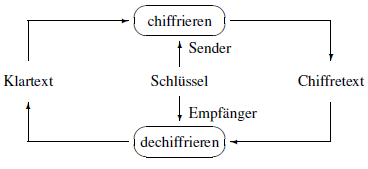
\includegraphics[width = 0.5 \textwidth]{Graphics/Cipher.png}
    \caption{Grundkonzept der Kryptographie}
    \label{konzept}
\end{figure}


In den 70er und 80er Jahren war die Kryptographie vor allem auf dem militären und diplomatischen Sektor beschränkt. Um geheime Nachrichten zu verschlüsseln, wurden sogenannte symmetrische Verschlüsselungsverfahren (z.B. Caesar-Verschlüsselung (\cite{moVarol})), wo nur ein gemeinsamer geheimer Schlüssel sowohl für die Ver- als auch für die Entschlüsselung benötigt wird, verwendet.

Aus diesem Grund ist es bei der symmetrischen Verschlüsselung sehr wichtig, dass der geheime Schlüssel auf einem sicheren Übertragungsweg an den Empfänger weitervermittelt wird, bevor die verschlüsselten Nachrichten übermittelt werden können. Früher wurde der Schlüssel meist persönlich, in Form eines Botens, übergeben. 
Da das persönliche Übergeben des Schlüssels sehrumständlich ist und es besteht das Risiko, dass der Schlüssel belauscht oder gestohlen werden konnte, wurden weitere Verschlüsslungsverfahren vorgeschlagen und zwar asymmetrisches Verschlüsselungsverfahren (auch Public-Key-Verfahren gennant) \cite{werner}. 

Im Gegensatz zu einem symmetrischen Verschlüsselungsverfahren erfordern asymmetrische Verschlüsselungsverfahren, nicht nur einen Schlüssel, sondern ein Schlüsselpaar bestehend aus einem öffentlichen Schlüssel und einem privaten Schlüssel \cite{damer}. Die Kommunikation erfolgt hier ohne vorhergehenden Schlüsselaustausch und ist jedoch viel langsamer als die Kryptografie mit privaten Schlüsseln. Mit dem privaten Schlüssel werden Daten entschlüsselt oder digitale Signaturen erzeugt, während mit dem öffentlichen Schlüssel Daten verschlüsselt und die Authentizität von erzeugten Signaturen überprüft  werden(\cite{sahuMa}; \cite{damer}). Die Abbildung \ref{key} veranschaulicht diese Schlüssel. 

\begin{figure}[!htb]
    \centering
    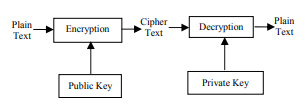
\includegraphics[width = 0.5 \textwidth]{Graphics/Fig1. Encryption.PNG}
    \caption{Public-Key Verschlüsselung}
    \label{key}
\end{figure}


Das erste asymmetrische Kryptosystem, Rivest-Shamir-Adleman-Verfahren (RSA-Verfahren) wurde im Jahr 1977 von Ronald Rivest, Adi Shamir und Leonard Adleman gefunden, 
danach wurden weitere Kryptosysteme wie Rabin, Elgamal, Diffie Hellman Schlüsselaustausch (DH) und Elliptische Kurven-Kryptogrphie vorgestellt.
Für unsere Arbeit liegt jedoch der Schwerpunkt auf der Kryptographie mit elliptischen Kurven und die Erzeugung von Schlüsseln, die für das Diffie-Hellman-Verfahren notwendig sind.


Die elliptische Kurvenkryptographie (ECC) ist Verschlüsselungstechnik mit öffentlichem Schlüssel, 
die auf der algebraischen Struktur elliptischer Kurven über endlichen Körper basiert \cite{mihNita} und zur Erstellung schnellerer, kleinerer und effizienterer kryptografischer Schlüssel verwendet werden kann \cite{khan}. 

Die Verwendung einer elliptischen Kurve in der Kryptographie wurde im Jahr 1985 unabhängig voneinander von Miller [10] und \cite{koblitz} vorgeschlagen. In den späten 1990er Jahren wurde ECC von einer Reihe von Organisationen wie ANSI [4, 5], IEEE [4,6], ISO [7, 8], NIST [9, 10] standardisiert und erhielt kommerzielle Akzeptanz \cite{GaMoDa}.
Das bekannteste Verschlüsselungsschema ist das Elliptic Curve Integrated Encryption Scheme (ECIES), das in IEEE- und auch in SECG SEC 1-Standards enthalten ist\cite{marKaur}. Beispiele für die Anwendung von ECC sind unter anderen Mehrzweck-Smartcards, die  neuen  deutschen  Personaldokumente\cite{merLo}, 

Im Allgemeinen basieren Kryptosysteme mit öffentlichem Schlüssel auf die Schwierigkeit der Lösung bestimmten mathematischen Probleme, z.B. beruht RSA-Verfahren auf dem Integer Factorizierungsproblem und DH sowie ECC basieren auf dem Diskreten Logarithmus-Problem. Es besteht jedoch ein Problem bei herkömmlichen Kryptosystemen mit öffentlichem Schlüsseln wie RSA. 

Das Hauptproblem besteht darin, dass die Schlüsselgröße ausreichend groß sein muss, um die Sicherheitsanforderungen auf hohem Niveau zu erfüllen, was zu einer geringeren Geschwindigkeit und einem höheren Bandbreitenverbrauch führt. Dies ist nicht den Fall, wenn elliptische Kurven (EC) für das Public Key Verfahren eingesetzt sind, da ECC im Vergleich zu RSA für den Benutzer eine gleichwertige Sicherheit bei kleineren Schlüsselgrößen bietet und für Angreifer schwerer exponentieller Zeitherausforderung, um in das System einzudringen\cite{GaMoDa}.


Laut einigen Forschern kann ECC mit einem 164-Bit-Schlüssel ein Sicherheitsniveau erreichen, für dessen Erreichung andere Systeme einen 1.024-Bit-Schlüssel benötigen\cite{khan}. Es stellte sich heraus, dass ECC das effizienteste Kryptosystem mit öffentlichem Schlüssel ist \cite{naRaj}.
Der Grund dafür ist, dass nach Miller und Koblitz das Diskreter-Logarithmus-Problem für elliptische Kurven schwerer sei als das klassische Diskreter-Logarithmus-Problem ist und zudem auch schnellere Laufzeiten ermögliche. Bevor das Diskreter-Logarithmus-Problem vorgestellt wird, ist es wichtig zu definieren, was unter einer elliptischen Kurven zu verstehen ist. 

Im Allgemeinen ist eine elliptische Kurve eine projektive, algebraische Kurve \textbf{C(K)}, auf der sich ein bestimmter Punkt O befindet, der als Punkt unendlich oder Nullpunkt bezeichnet wird \cite{GaMoDa}.


Eine elliptische Kurve E über ein Körper $ K $ der Charakteristik $ \neq $
2 oder 3, lässt sich formal definieren als die Menge der Punkte
$ (x, y) $ $ \in $ \( K \)  der Weierstraß-Gleichung:

\begin{ceqn}

\begin{equation}
       y^2 = x^3 + ax + b \quad 
       \text{ mit a, b $ \in $ $ K $           \cite{koblitz}.}
\end{equation} 

\end{ceqn}

Elliptische Kurven in Form von Gleichungen können in singuläre und nicht-singuläre Gruppen unterteilt werden. In der ECC werden nicht-singuläre Kurven bevorzugt, damit eine Kurve frei von Spitzen oder Selbstüberschneidungen sein kann\cite{razad}.

Eine elliptische Kurve wird als \textit{nicht-singulär} bezeichnet,
wenn sie keinen Punkt $ P = (x, y) $ enthält, an dem ein mathematisches Objekt nicht definiert ist \cite{werner} und für die Werte a und b folgende Bedingung
 $ \Delta = 4a + 27b \neq 0 $
 erfüllt, um eine endliche Abelsche Gruppe zu bilden. 
 
In der abstrakten Algebra ist eine abelsche Gruppe, eine Gruppe, in der das Ergebnis der Anwendung der Gruppenoperation auf zwei Gruppenelemente nicht von ihrer Reihenfolge abhängt.


Die \textbf{Charakteristik} eines Körpers $ \mathbf{K} $ ist die kleinste positive Zahl \textbf{p} mit 
\begin{ceqn}
\begin{align*}
   \underbrace{1 \cdot 1 \cdot 1 \cdot \ldots \cdot 1}_{\text{$k$ mal} } = 0   \quad \text{, falls sie existiert.}
\end{align*}
\end{ceqn}
 
Dies ist beispielsweise für die Körper der rationalen Zahlen $ \mathbb{Q} $, der reelen Zahlen $ \mathbb{R} $ und der komplexen Zahlen $\mathbb{C} $ der Fall.Für jeden endlichen Körper ist die Charakteristik immer eine Primzahl \cite{damer}.

$ \mathbf{K} $ kann ein beliebiger Körper, also etwa $ \mathbb{R} $, $ \mathbb{Q} $, $ \mathbb{C} $ oder ein endlicher Körper $ \mathbb{F} $ sein\cite{werner}. Die obige Gleichung entspricht die Definition einer elliptischen Kurve über reelen Zahlen.
Obwohl eine elliptische Kurve über den reellen Zahlen ein guter Ansatz ist, um die Eigenschaften einer elliptischen Kurve zu verstehen, erfordert sie eine höhere Rechenzeit, um verschiedene Operationen auszuführen, und ist manchmal aufgrund von Rundungsfehlern ungenau. Kryptographie-Schemata erfordern jedoch eine schnelle und präzise Arithmetik\cite{razad}. Folglich werden in kryptografischen Anwendungen zwei Arten von elliptischen Kurven verwendet:
	\begin{itemize}
	    \item Primzahlen über einem Feld $ \mathbf{Z_p} $, wobei p eine Primzahl und p > 3 ist. Alle Variablen und Koeffizienten werden aus einer Menge von ganzen Zahlen von 0 bis p - 1 entnommen und Berechnungen werden über Modulo p durchgeführt \cite{werner}.
        \item 	Binäre Kurve über dem Galois-Feld $ 2^m $, auch bekannt als $ GF(2^m) $, wobei alle Variablen und Koeffizienten in $ GF $ sind und Berechnungen über $ GF(2^m) $ durchgeführt werden.
	\end{itemize}

Da Primkurven analog zur Binärkurve keine erweiterte Bit-Fidding-Operation haben, sind sie für die Software-Implementierung geeignet\cite{razad}.



In dieser Arbeit wurde die Implementierung von elliptischen Kurven über endliche Körper mit $ \mathbf{K} $ = $ \mathbf{Z_p} $ berücksichtigt. Dazu wird mehr im Kapitel 4 erläutert.
Eine elliptische Kurve über dem endlichen Feld $ \mathbf{Z_p} $ enthält alle Punkte $ (x, y) $ in der $ \mathbf{Z_p} $ $ \times $ $ \mathbf{Z_p} $ Matrix, die die folgende elliptische Kurvengleichung erfüllt: 

\begin{ceqn}

\begin{equation}
     y^2 = x^3 + ax + b  \quad (mod p)
     \label{curve}
\end{equation}

\end{ceqn}

Dabei sind x und y Zahlen in $ \mathbf{Z_p} $  und ähnlich wie im realen Fall ist $ \Delta \neq $ 0.
Alle Punkte $ (x, y) $, die die obige Gleichung  erfüllen, liegen auch auf der elliptischen Kurve. Der öffentliche Schlüssel ist ein Punkt in der Kurve und der private Schlüssel ist eine Zufallszahl. Das Hinzufügen von Punkten auf der elliptischen Kurve ist jedoch kein einfacher Prozess, sondern an ein auf polynomiale Zeit zu lösendem Problem gebunden \cite{mo2014}: Das diskrete Logarithmusproblem. 


\section{Diskretes Logarithmusproblem }

Nehmen wir nun an, dass (G, $ \times $ ) eine multiplikative zyklische Gruppe mit Domainparametern g, h und n ist. 
Das \textbf{diskrete Logarithmusproblem} ist explizit definiert, als das Problem der Bestimmung einer eindeutigen Ganzzahl $ x $, die zufällig aus dem Intervall [1, p - 1] ausgewählt wird, so dass es gilt:

\begin{ceqn}

\begin{align*}
    g^x = h mod p
\end{align*}

\end{ceqn}
vorausgesetzt, dass eine solche ganze Zahl existiert.
Der Parameter $ g $ ist die Basis des Logarithmus bzw. ein Erzeuger der Gruppe $ \mathbf{G} $ ; $ n $ die Anzahl der Elemente in $ \mathbf{G} $ ; der private Schlüssel bzw. das diskrete Logarithmusproblem von $ h $ zur Basis $ g $  ist die Ganzzahl $ x $, und der öffentliche Schlüssel ist   $ h = g^x $ \cite{Hankerson}.


Das \textbf{Elliptic Curve Diskrete Logarithmus Problem (ECDLP)} ist ähnlich definiert, aber betrachtet die Weierstraß-Gleichung für eine elliptische Kurve $ \mathbf{E:} $ $ y^2 = x^3 + ax + b $ über $ \mathbb{Z_p} $ und zwei Punkte $ P $ und $ Q $ $\in $ $ \mathbf{F_p} $.  Zu bestimmen ist, eine Zahl k $ \in $ $ \mathbf{Z} $ mit

\begin{ceqn}
\begin{align*}
      Q = kP  \quad \text{, falls so ein k existiert.}
\end{align*}
   
\end{ceqn}

Die Primzahl p, die Gleichung der elliptischen Kurve E und der Punkt P und seine Ordnung n sind die Domainparameter. Der privater Schlüssel ist die ganze Zahl k, die gleichmäßig zufällig aus dem Intervall [1, n - 1] ausgewählt wird, und der entsprechende öffentliche Schlüssel ist $ Q = kP $.


Das Lösen von ECDLP ist viel schwieriger als DLP, da die Komplexität der Punktarithmetik in ECDLP im Vergleich zur Ganzzahlarithmetik in DLP zunimmt. 
Aus diesem Grund ist ECC in der Lage, ein ähnliches Sicherheitsniveau wie RSA bereitzustellen, jedoch mit einer kürzeren Schlüsselgröße, was es wiederum zur beliebtesten Wahl macht\cite{mo2014}. 

Damit ein auf $ \mathbf{F_p} $basierendes diskretes Logarithmus-System effizient ist, sollten schnelle Algorithmen zur Berechnung der Gruppenoperation bekannt sein. Aus Sicherheitsgründen sollte das Problem des diskreten Logarithmus in $ \mathbf{Z_p} $ unlösbar sein\cite{Hankerson}.
Es gibt viele Algorithmen zur Lösung von \textbf{ECDLP}, aber der erfolgreichste ist die Kombination von Pollards Rho- und Pohlig-Hellman-Angriffen mit vollständig exponentieller Laufzeit (\cite{mo2014};\cite{Hankerson}). 
Angriffe resultieren normalerweise aus den Schwächen bei der Auswahl der elliptischen Kurve und des endlichen Feldes (siehe Kapitel 4 und 5), aber die meisten Angriffe können durch korrekte Auswahl der Parameter der elliptischen Kurve vereitelt werden \cite{mo2014}.
Daher sollten diese öffentlichen Parameter sicher ausgewählt werden, um alle erkannten Angriffe zu vermeiden\cite{aliKa}. Der nächste Abschnitt beschäftigt sich näher mit diesen Parametern. 

\section{Domänenparameter für elliptischen Kurven}

Vor der Implementierung eines ECC-Systems müssen mehrere Entscheidungen getroffen werden.
Dazu gehören die Auswahl von Domänenparametern für elliptische Kurven (zugrunde liegendes endliches Feld, Felddarstellung, elliptische Kurve) sowie Algorithmen für Feldarithmetik, elliptische Kurvenarithmetik und Protokollarithmetik. 
Die Auswahl kann durch Sicherheitsaspekte, Anwendungsplattform (Software oder Hardware), Einschränkungen der jeweiligen Computer- und Kommunikationsumgebung (z. B. Speichergröße, Bandbreite) beeinflusst werden \cite{Havaze}.

Im Allgemeinen können zwei Arten von elliptischen Kurvendomänenparametern verwendet werden \cite{standard}:
\begin{itemize}
    \item elliptische Kurvendomänenparameter über $ \mathbf{Z_p} $ und
    \item elliptische Kurvendomänenparameter über $ \mathbf{F_2^m} $ .
\end{itemize}

\subsection{Parameter über \texorpdfstring $ \mathbf{ Z_p } $ }

Die Domänenparameter für die elliptische Kurve über $ \mathbf{F_p} $ sind  ein Sextuple
\begin{ceqn}
\begin{align*}
  (p, a, b, G, n, h)  
\end{align*}
\end{ceqn}
 bestehend aus einer ganzen Zahl $ \mathbf{ p } $, die das endliche Feld $ \mathbf{ Z_p} $ spezifiziert; der Kurve aus \ref {curve}, den Parametern a und b, einem Basispunkt $  G = (x_G, y_G) $ auf $ E(\mathbf{Z_p}) $,  $ \mathbf{ n } $ die Ordnung der elliptischen Kurve und dem Cofaktor h, wobei 
 \begin{ceqn}
 \begin{align*}
   h = \frac{ \#E ({F_p}) }{ n } 
 \end{align*} 
 \end{ceqn}
und $ \#E (\mathbf{F_p}) $  die Anzahl der Punkte auf einer elliptischen Kurve ist.(\cite{standard}; \cite{GaMoDa})


\subsection{Parameter über \texorpdfstring $ \mathbf{F_2^m} $  }
Die Domänenparameter für die elliptische Kurve über $ \mathbf{ F_2^m } $ sind ein Septuple
\begin{ceqn}
\begin{align*}
           T = (m, f (x), a; b; G; n; h) 
\end{align*}
\end{ceqn}
bestehend aus einer ganzen Zahl $ m $, einem irreduziblen binären Polynom $ f (x) $ vom Grad m, Parameter a, b $ \in $ $ \mathbf{ F_2^m} $ der durch die Gleichung der elliptischen Kurve $ \mathbf{ E (F_2^m) } $:
\begin{ceqn}
\begin{equation}
           y^2 + xy = x^3 + ax^2 + b  \quad \in F_2^m
\end{equation}
\end{ceqn}
definiert sind, einem Basispunkt $ G = (xG; yG) $ auf $ E (F_2^m) $, eine Primzahl n, die in der Größenordnung von G liegt und die Cofaktor h mit 
\begin{ceqn}
 \begin{align*}
   h = \frac{ \#E ({F_p}) }{ n } 
 \end{align*} 
 \end{ceqn}
und $ \#E (\mathbf{F_p}) $  die Anzahl der Punkte auf einer elliptischen Kurve ist. (\cite{standard}; \cite{GaMoDa})
Für diese Arbeit wurden jedoch nur Parameter über $ \mathbf{ Z_p } $ bevorzugt. 

Je nach gewähltem Feld verwendet ECC für seine Operationen modulare Arithmetik oder Polynomarithmetik. Dies wird im nächsten Kapitel(Kapitel 3) präsentiert. 



\cleardoublepage\chapter{Zahlentheoretische Grundlagen}

Aufgrund vielversprechender Ergebnisse in verschiedenen Sicherheitsanwendungen ist es sehr wichtig, elliptische Kurvenarithmetik und ECC-basierte Kryptosysteme zu verstehen. wichtige Grundlagen
der Zahlentheorie, die für die Kryptographie von Bedeutung sind, werden hier
zusammengefasst. Es handelt sich dabei um die modulare Arithmetik, Die Verwendung der elliptischen Kurvenarithmetik macht ECC unter allen vorhandenen kryptografischen Schemata einzigartig. Die Arithmetik verwendet modulare Arithmetik, einschließlich modularer Multiplikation, Addition und die Bestimmung
von modularen Inversen. In diesem Kapitel werden endliche Feldarithmetikoperationen wie modulare Addition, modulare Subtraktion, modulare Multiplikation und modulare Inversion zusammen mit Beispielen beschrieben.

\section{Modulararithmetik}



\section{Modulare Inverse}



\section{Polynomarithmetik}
\cleardoublepage\include{Chapters/Endliche_Körper}
\cleardoublepage\chapter{Elliptische Kurven}



\section{Darstellungen von Punkten}
Um Punkte auf einer elliptischen Kurve darzustellen oder anzugeben gibt es mehrere Möglichkeiten, die unterschiedliche Vor- und Nachteile haben. Jede Darstellung wird daher auch anders miteinander verrechnet.
\subsection{Affine Darstellung}
Die affine Darstellung ist die gebräuchlichste Art und Weise einen Punkt und eine elliptische Kurve darzustellen, da es nur die x und y Koordinaten gibt.\\
In diesem Fall gibt es keine einheitliche Darstellung der Unendlichkeit und man muss prüfen, ob die Koordinaten auf der Kurve \[y^2 = x^3 + Ax + B\] liegen.
\subsection{Projektive Darstellung}
Bei der projektiven Darstellung kommt die z - Koordinate hinzu, sodass aus der zwei-dimensionalen eine drei-dimensionale Kurve entsteht. Die Umrechnung eines affinen Punktes in einen projektiven Punkt ist dabei einfach durch das Hinzufügen von z = 1 durchzuführen. Bei der umgekehrten Richtung muss man die x und y Koordinaten durch z teilen, woraus folgt, dass alle Punkte mit z = 0 nicht auf der Kurve liegen und unendlich sind. Zur Erinnerung, die Formel der Kurve ändert sich von \(y^2 = x^3 + Ax + B\) zu \[y^2z = x^3 + Axz^2 + Bz^3\]\\
Eine Punktaddition benötigt zwölf Multiplikationen und zwei Quadrierungen, während eine Punktverdopplung nur sieben Multiplikationen und fünf Quadrierungen braucht \cite{Washington2003}.
\\
\subsection{Jacobi Darstellung}
Um einen noch größeren Speedup zu erreichen, kann man Jakobi Koordinaten verwenden, da diese besonders effizient beim Verdoppeln sind. Hier ist die Darstellung (x,y,z) bei der Kurvenform \[y^2 = x^3 + Axz^4 + Bz^6\] gewählt. Zum Konvertieren nach affin muss man folgende Rechnung \((x/z^2, y/z^3)\) anwenden. Der Punkt unendlich ist mit (1,1,0) definiert. Natürlich werden alle anderen Punkte, die nicht auf der Kurve liegen auch als unendlich behandelt \cite{Washington2003}.

\subsection{k-fache Punktmultiplikation}
Wenn ein Punkt mit k multipliziert wird, unterscheidet man, dass bei \(k > 0\) \[P + P + ... + P = kP\] und bei \(k < 0\) \[ (-P) + (-P) + ... + (-P) = kP\] berechnet wird. Durch wiederholtes Verdoppeln erreicht man bei großen \(k\) die beste Performance und da die elliptischen Kurven auf endlichen Feldern basieren, muss man sich auch keine Gedanken um immer größere Koordinaten machen, da diese immer \( mod p\) gerechnet werden \cite{Washington2003}. Der Algorithmus sieht wie folgt aus:

\begin{table}[!ht]
\centering
	\begin{tabular}{l}
		\toprule
		\textbf{Algorithmus: k-fache Punktmultiplikation}\\
		\midrule
		Sei k eine positive natürliche Zahl und P ein beliebiger Punkt auf der elliptischen Kurve\\ e. Dann wird \(kP\) wie folgt berechnet:\\
		1. \(a = k , B = \infty , C = P\)\\
		2. wenn a gerade, dann \(a = a/2 , B = B , C = 2C\)\\
		3. wenn a ungerade, dann \(a = a - 1 , B = B + C , C = C\)\\
		4. wenn \( a \neq 0\), gehe zu 2.\\
		5. return B\\
	   \bottomrule
	\end{tabular}
	\caption{Algorithmus: k-fache Punktmultiplikation \cite{Washington2003}}
	\label{tab6}
\end{table}


\subsection{Negation}
Die Negation wird durch einen Vorzeichenwechsel durchgeführt bei der y-Koordinate \cite{Washington2003}. Da die Zahl dann negativ ist, muss noch das positive Gegenstück im endlichen Zahlenraum gefunden werden, was durch die einfache Addition der Zahl p geht. Vorausgesetzt ist hierbei eine affine Darstellung. Kommt man von einer anderen Darstellung muss man zuerst zur affinen Darstellung, dann negieren und abschließend in die ursprüngliche Darstellung umrechnen.

\section{Punktaddition}
\subsection{affin}
Die Addition zweier Punkte bedeutet, dass man eine Gerade durch die Punkte zieht und diese Gerade schneidet die Kurve in einem dritten Punkt, dieser ist das Ergebnis.\\
Bei zwei unterschiedlichen Punkten, wovon einer nicht im unendlichen Bereich liegt, wird die Steigung durch den Differenzquotienten berechnet: \[m = \frac{x_1-x_2}{y_1 - y_2}\]
Nun braucht man nur noch einzusetzen \[x = m^2 -x1 - x2\] \[y = m(x-x_1)-y_1\] und erhält den neuen Punkt.\\
Wenn \(P_1 = P_2\) ist, dann hat man eine Senkrechte durch \(P_1\), die die Kurve an einer Stelle \(P_3\) schneiden muss. Diesen Punkt erhält man durch folgende Formeln:\\

Ansonsten gilt \(P_1 + \infty = P_1\) , wobei \(\infty\) ein Punkt außerhalb der Kurve ist \cite{Washington2003}.\\
Die Addition ist für den Rechner bei großen Zahlen sehr aufwendig, da man dividieren muss und das die anspruchsvollste Rechenoperation ist. Man benötigt zwei Multiplikationen, eine Quadrierung und eine Division \cite{Washington2003}.
\subsection{projektiv}
Bei \(P_1 \neq \pm P_2\) sieht die Addition wie folgt aus:
\[u = y_2z_1 - y_1z_2\] \[v = x_2z_1 - x_1z_2\] \[w = u^2z_1z_2 - v^3 -2v^2x_1z_2\] \[x_3 = 2uw\] \[y_3 = t(4v -w)-8y_1^2u^2\] \[z_3 = 8u^3\]
\subsection{jakobi}
Bei zwei unterschiedlichen Punkten wird wie folgt addiert:
\[r = x1z_2^2\] \[s = x_2z_1^2\] \[t = y1z_2^3\] \[v = s - r\] \[w = u - t\] \[x_3 = -v^3 - 2rv^2 + 2^2\] \[y_3 = -tv^3 + (rv^2-x_3)*w_1\] \[z_3 = vz_1z_2\]
Dadurch ergeben sich zwölf Multiplikationen und vier Quadrierungen.\\
Ein weiterer Vorteil dieser Darstellung ist die Kompatibilität zu affinen Punkten. Hier benötigt man für die Addition von einem Jacobi Punkt und einem affinen Punkt nur acht Multiplikationen und drei Quadrierungen \cite{Washington2003}.


\section{Punktverdopplung}
\subsection{affin}
Falls \(P_1 = P_2\) ist, dann erhält man eine Senkrechte durch \(P_1\), die die Kurve an einer Stelle \(P_3\) mit einer Steigung \[m = \frac{3x^2+A}{2y}\] schneiden muss.\\
Daraus wird wiederum die x Koordinate \[m^2-2x\] und y Koordinate berechnet \[y = m(x - x_0)+y\]\\ Einerseits bekommt man in dieser Darstellung den Bruch nicht aufgehoben und daher ist sie nicht effizient berechenbar, aber andererseits ist es die für den Menschen anschaulichste Notation. Aus diesem Grund konvertieren wir die meisten Punkte zur Ausgabe in diese Darstellungsform, nachdem wir über eine der zwei folgenden Arten die Punktverdopplung durchgeführt haben.
\subsection{projektiv}
Wenn man zwei gleiche Punkte addiert, ändert sich die oben genannte Formel zu:
\[t = Az_1^2 + 3x_1^2\] \[u = y_1z_1\] \[v = ux_1y_1\] \[w = t^2 - 8v\] \[x_3 = 2uw\] \[y_3 = t(4v-w)- 8y_1^2u^2\] \[z_3 = 8u^3\] mit dem Sonderfall von \(P1 = -P2\) folgt \(P1 + P2 = \infty\). Eine Punktverdopplung benötigt nun nur noch sieben Multiplikationen und fünf Quadrierungen.
\subsection{jakobi}
Verdoppelt man einen Punkt, erkennt man direkt im Vergleich die Einfachheit der Formel:
\[v = 4x_1y_1^2\] \[w = 3x_1^2 + Az_1^4\] \[x_3 = -2v + w^2\] \[y_3 = -8y_1^4 + (v-x_3)w_1\] \[z_3 = 2y_1z_1\]\\ 
Wodurch man die Operationen auf drei Multiplikationen und sechs Quadrierungen reduzieren kann. Das ist besonders schnell berechenbar für einen Computer \cite{Washington2003}.\\
Wenn man nun noch den Fall betrachtet, dass \(A = -3\) ist, wird \[w = 3(x_1^2 - z_1^4 = 3(x_1 + z_1^2)(x_1 - z_1^2)\] mit nur einer Multiplikation und einer Quadrierung, statt mit drei Quadrierungen berechnet. Daher haben viele Kurven in NIST Listen auch den Faktor \(A = -3\).
\cleardoublepage\chapter{Elliptic Curve Diffie Hellman}
\cleardoublepage\chapter{Fazit}

\section*{Annick:}
Da ich noch keine Berührung mit endlichen Körpern und modularer Arithmetik hatte, war auch die Elliptische Kurve mathematisches Neuland für mich, sodass ich einen schweren Start in dieses Projekt hatte. Ich musste zuerst einiges Wissen recherchieren und nachlesen um dann meine Klassen implementieren zu können. Daher bin ich sehr zufrieden, dass das recht reibungslos geklappt hat und unsere Klassen und Methoden ohne größere Probleme miteinander kompatibel waren. 


\section*{Richard:}
Das Projekt ist außerordentlich interessant. Da ich schon ein Semester Kryptographie hatte, 
ist die Elliptische Kurve kein Fremdwort mehr. Die Probleme die anfänglich und während des Projektes auftraten, waren schlechtes Zeitmanagement und Kommunikationsprobleme.
Diese sind durch einige Wahlpflichtfächer mit großen Anforderungen und auch wegen der Pandemie, die ein regelmäßiges persönliches Treffen unmöglich machte, zu erklären.\\
\\
Dennoch haben wir das beste daraus gemacht. Die größte Schwierigkeit in diesem Projekt war der Anfang des Projektes.
\\
Alle mussten auf dem gleichen Stand sein, so dass keine neuen Probleme mit dem Thema entstehen.
Je mehr organisatorische Probleme gelöst wurden, desto weniger Konflikte entstanden.
\\
\\
In meinen Teil waren der Fermat-Test und die endlichen Körper relativ schnell gelöst.
Diese sind nicht so kompliziert wie man auf den ersten Blick denkt.\\
Lediglich war die Primzahlpotenz sehr komplex, denn zuerst hatte ich die falsche Quellen genommen und dadurch das Thema falsch verstanden.\\
Dies hat dazu geführt, das ich das Kapitel komplett neu machen musste, jedoch lernte ich schnell dazu und somit hatte ich eine neue Grundlage um das Kapitel aufzubauen.\\
\\
Zuerst musste man verstehen, das es nur Polynome berechnet werden und kein richtiger Wert erwartet wird. 
Natürlich wird man neugierig und will viel mehr machen, jedoch hat alles eine Zeitgrenze und es wurden nur die Grundlagen implementiert.\\
\\
Dieses Projekt hat mein persönliches Interesse an die Mathematik der Kryptographie geweckt. 

\section*{Hendrik:}
Ähnlich wie Richard hatte ich mich schon vor dem Projekt mit dem Thema Elliptische Kurven beschäftigt. Daher fiel es mir mehr oder weniger leicht die Implementierung der verschiedenen Darstellungen zu implementieren. Besonders die Mathematik hinter der Punktaddition und die daraus resultierenden SpeedUps faszinieren mich. Hinzu kommt das Phänomen, dass man mit jeder Iteration der Punktaddition wieder einen Punkt auf der Kurve trifft und dadurch einen sicheres Verfahren für einen Schlüsselaustausch bereitstellt.\\
Natürlich gab es auch kleinere Probleme während der Projektzeit, aber die sind für mich nebensächlich, da ich einen guten Gesamteindruck von unserer Teamarbeit habe. Schließlich haben wir alle gut zusammengearbeitet und können ein ordentliches Programm vorweisen.


%\cleardoublepage\include{Chapters/Handbuch}
%\cleardoublepage%*****************************************
\chapter{Beispiele}\label{ch:examples}
%*****************************************

%************************************************
%*  Abkürzungen *********************************
%************************************************

\section{Abkürzungen}

Um Abkürzungen zu verwenden, muss über \lstinline|\usepackage{acronym}| das benötigte Package geladen werden. Danach kann man lange Begriffe ganz bequem abkürzen:

So muss man nicht ständig \ac{WLAN} ausschreiben, auch \ac{TCP} lässt sich abkürzen. Würde man im Text \acs{WLAN} oft verwenden, kann man sie, wie hier, nur als
Abkürzung anzeigen lassen - oder bei Bedarf die Erklärung mitliefern (\acf{WLAN}). Weiteres Beispiel könnte die \ac{GoF} sein.

Weitere Informationen sind im \href{http://www.ctan.org/tex-archive/macros/latex/contrib/acronym}{Acronym-Manual} zu finden.
%*********************************************
%*	Biblatex-Beispiel
%*********************************************
\section{Beispiel für BibLaTeX}

BibLaTeX ist ein Package, das einem die Arbeit mit Zitaten bzw. Quellenangaben erleichtern kann. Mit JabRef (\autoref{sec:Werkzeuge}) ist es möglich
\textit{*.bib}-Dateien zu erstellen, in denen alle Angaben zu Autor, Buchtitel, Erscheinungsdatum usw. hinterlegt werden, welche zum passenden Zeitpunkt
abgerufen werden können. Das Literaturverzeichnis wird mittels \lstinline{\printbibliography} ausgegeben.

Im Allgemeinen wird im Literaturverzeichnis auch nur jene Literatur aufgenommen, die auch in der \textit{*.tex}-Datei referenziert wird. Danach ist es wichtig
nicht nur mit \textit{Pdf\-LaTeX}, sondern auch mit \textit{BibLaTeX} zu kompilieren, damit die zitierten Einträge in die verschiedenen Hilfsdateien aufgenommen
werden können. %Hinweis: Pdf\-LaTeX teilt LaTeX mit, dass nur zwischen Pdf und LaTeX getrennt werden darf


\subsection*{Einige Zitate}
In diesem Satz könnten wir auf \cite{knuth:1976} verweisen, ebenso auf das wichtige Werk \cite{dueck:trio}. Wenn uns das nicht genug ist, sollten wir das anmerken,
was in \cite{sommerville:1992} geschrieben wurde. Im Zweifelsfall verweisen wir auf eine einzelne Seite, wie in \cite[112]{bentley:1999} zu finden. 

Üblicherweise wird auch der Name des Autors bzw. der Autoren genannt, also beispielsweise bei einem Verweis auf \citeauthor{knuth:1976} \cite{knuth:1976} oder 
auch bei mehreren Autoren \citeauthor{cormen:2001} \cite{cormen:2001}. LaTeX stellt Mechanismen zur Verfügung, auch dies automatisiert zu erledigen.





\section{Referenzierungen}
Mit Referenzierungen kann ich ganz bequem auf Textpassagen, Kapitel, Sections oder Abbildungen im weiteren Text verweisen.
Dies ist ein Verweis auf \autoref{subsec:Beispieltext}, der sich auf \autoref{subsec:Beispieltext} befindet.

Auch ein Verweis auf \autoref{tab:beispieltabelle1} auf Seite~\pageref{tab:beispieltabelle1} ist möglich.

Man sollte beachten, dass man sein Dokument, wenn es Referenzierungen enthält, mehrmals kompiliert, da sonst manche
Verweise nicht aufgelöst werden können.


\subsection{Beispieltext}\label{subsec:Beispieltext}
\blindtext

\section{Dateien einbinden}

Damit man nicht alle Einstellungen, Optionen, Packages und Texte, Abbildungen etc. in einer Datei unterbringen muss, werden
zwei Befehle bereitgestellt, um externe \textit{*.tex}-Dateien einzubinden: \lstinline|\include{PFAD}| und \lstinline|\input{PFAD}|.
Mit dem erstem Befehl wird eine neue Seite angelegt, danach kommen die Inhalte aus der angegebenen Datei; mit dem zweiten
Befehl wird keine neue Seite angelegt -- der Inhalt der angegebenen Datei wird direkt an die betroffene Stelle eingefügt.

\textbf{Wichtig:} Der \textit{Pfad} wird sinnigerweise \textit{relativ} angegeben, wobei als Stammverzeichnis jenes Verzeichnis
angesehen wird, in dem die \textit{*.tex}-Datei mit der \textit{Document}-Umgebung abgelegt ist (in diesem Fall ist es 
\textit{htwsaar-i-mst-config.tex}).
%************************
%*		Tabellen 		*
%************************

\section{Tabellen}
\label{sec:Tabellen}

\subsection{Einfache Tabelle}
In LaTeX lassen sich Tabellen unterschiedlicher Ausprägung einfach erzeugen. Das allgemeine Format einer Tabelle sieht aus wie folgt:

\begin{lstlisting}[caption={Allgemeines Format}]
\begin{table}
	\caption{BESCHRIFTUNG}
	\begin{tabular}{FORMATIERUNG}
		TABELLENINHALT
	\end{tabular}
\end{table}
\end{lstlisting}

Eine Beispieltabelle (Tabelle \ref{tab:beispieltabelle1}) könnte also so aussehen:

\begin{lstlisting}[caption={Tabelle \ref{tab:beispieltabelle1}}]
\begin{table}
	\caption{Beispiel 1}
	\begin{tabular}{lrcr}
		\toprule
		\textbf{Name} & \textbf{Vorname} & \textbf{Matrikelnummer} & \textbf{Lieblingsspeise}\\
		\midrule
		Jackson & Michael & 123456 & Erdbeereis \\
		Springsteen & Bruce & 234567 & Schwedisches Lakritz \\
		Bach & Anna, Magdalena & 3456789 & Frankfurter Kranz \\
		Schumann & Clara & 4567890 & Bisquitt\"ortchen \\
		\bottomrule
	\end{tabular}
	\label{tab:beispieltabelle1}
\end{table}
\end{lstlisting}

Mit \lstinline|\caption{Beispiel 1}| bekommt unsere Tabelle eine Beschriftung am Tabellenkopf. \lstinline{l|r|c|r} legt die Textausrichtung der einzelnen Spalten fest: \lstinline|l| bedeutet linksausgerichtet, \lstinline|r| rechtsausgerichtet und \lstinline|c| zentriert. Durch \lstinline{|} werden Spaltenlinien gezogen. \lstinline|\toprule|, \lstinline|\midrule| und \lstinline|\bottomrule| erzeugen Kopf-, Mittel- und Abschlusslinie in der Tabelle. Als Spaltentrenner wird das \lstinline{&} genutzt, Zeilentrenner ist der doppelte Backslash (\lstinline|\\|). Am Ende kann die Tabelle auch mit einem Label versehen werden (\lstinline|\label{tab:beispieltabelle1}|), über welches diese referenziert wird.

%\begin{center}
\begin{table}[b]
	
	\caption{Beispiel 1}
	\begin{tabular}{lrcr}
		\toprule
		\textbf{Name} & \textbf{Vorname} & \textbf{Matrikelnummer} & \textbf{Lieblingsspeise}\\
		\midrule
		Jackson & Michael & 123456 & Erdbeereis \\
		Springsteen & Bruce & 234567 & Schwedisches Lakritz \\
		Bach & Anna, Magdalena & 3456789 & Frankfurter Kranz \\
		Schumann & Clara & 4567890 & Bisquittörtchen \\
		\bottomrule
	\end{tabular}
	\label{tab:beispieltabelle1}
\end{table}
%\end{center}

\subsection{Erweiterte Tabellenbefehle}
Um Tabellen in LaTeX flexibler zu gestalten gibt es weitere Befehle bzw. zusätzliche Pakete, die einem das Leben leichter machen (Tabelle \ref{tab:beispieltabelle2}). Hierzu ein weiteres Beispiel:

\begin{lstlisting}[caption={Tabelle \ref{tab:beispieltabelle2}}]
\begin{table}
	\centering
	\caption{Beispiel 2}
	\begin{tabular}{lll}
		\hline
		Author & Title & Year \\
		\hline
		\hline
		\multirow{3}{*}{Stanislav Lem} & Solaris & 1961 \\
 			& Roboterm\"archen & 1967 \\
 			& Der futurologische Kongress & 1971 \\
		\hline
		\multirow{3}{*}{Isaac Asimov} & Ich, der Robot & 1952 \\
 			& Der Tausendjahresplan & 1966 \\
 			& Doctor Schapirows Gehirn & 1988 \\
		\hline
	\end{tabular}
\label{tab:beispieltabelle2}
\end{table}
\end{lstlisting}

Mit \lstinline|\centering| wird die Tabelle zentriert ausgerichtet, analoge Befehle für rechts- bzw. linksausrichtung sind z.B. \lstinline|\raggedleft| und \lstinline|\raggedright|. \\

Eine weitere Form der Tabellen ist das Package \textit{tabularx}, das variable Spaltenbreiten unterstützt, und \textit{booktabs}, welches mit horizontalen Linien besser arbeiten kann.
\begin{table}
	\centering
	\caption{So sollte man es nicht machen! Beispiel für einen schlechten Tabellenstil}
	\begin{tabular}{|l|l|l|}
		\hline
		Author & Title & Year \\
		\hline
		\hline
		\multirow{3}{*}{Stanislav Lem} & Solaris & 1961 \\
 			& Robotermärchen & 1967 \\
 			& Der futurologische Kongress & 1971 \\
		\hline
		\multirow{3}{*}{Isaac Asimov} & Ich, der Robot & 1952 \\
 			& Der Tausendjahresplan & 1966 \\
 			& Doctor Schapirows Gehirn & 1988 \\
		\hline
	\end{tabular}
\label{tab:beispieltabelle2}
\end{table}
\section{Abbildungen}
%=============================

\textit{LaTeX} unterstützt generell die Formate \textit{*.jpeg}, \textit{*.png} und \textit{*.pdf}.
Handelt es sich z.B. um Strichgrafiken oder skalierbare Farbflächen, sollte \textit{*.pdf} die erste Wahl sein,
da sich in diesem Format Vektorgrafiken ohne Qualitätsverlust darstellen bzw. skalieren lassen.

\begin{figure}[bth] 
  \centering
  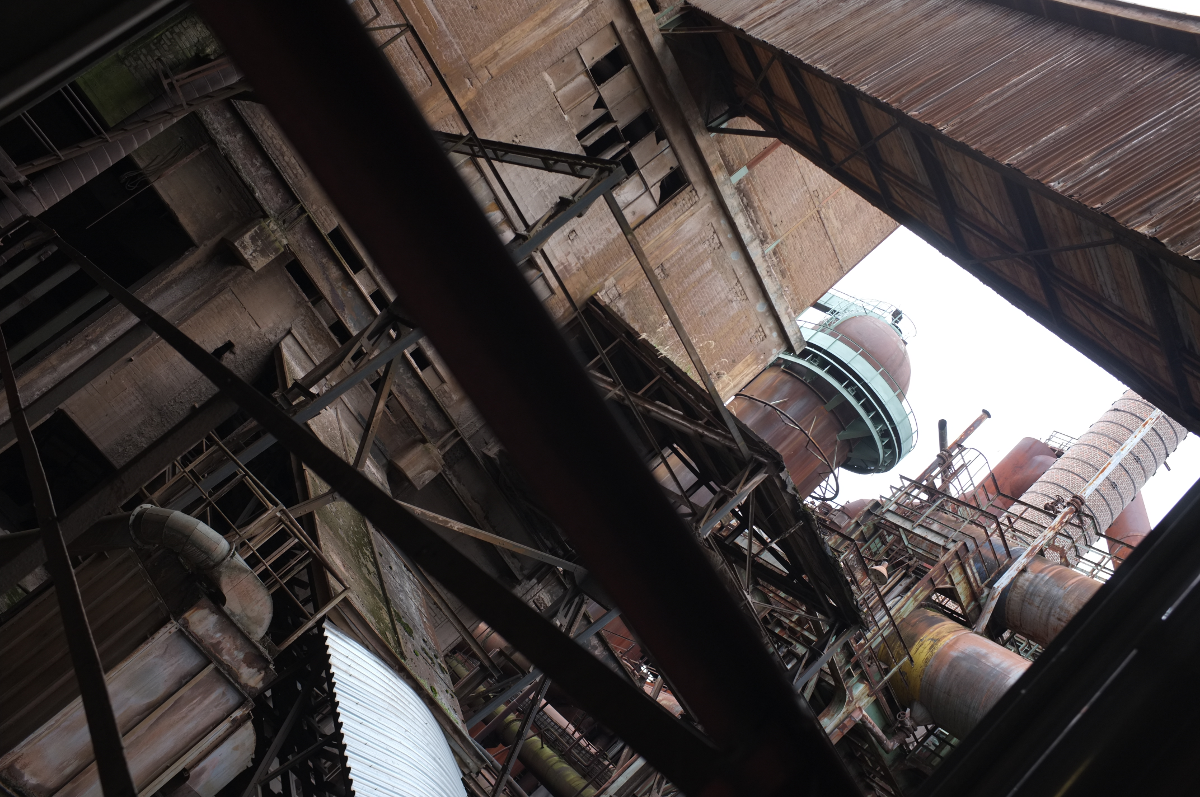
\includegraphics[width=0.7\textwidth]{Examples/example_5.png}
  \caption{Erstes Bild, Völklinger Hütte}
  \label{fig:Huette}
\end{figure}


\subsection{Wrapfigure}
Abbildung~\ref{fig:Huette} ist zwar ganz nett anzusehen, aber vielleicht sähe es eleganter aus, wenn die Abbildung 
von unserem Textabschnitt umflossen werden würde. Diese Art von Abbildungen sollte jedoch sparsam und mit großer Sorgfalt eingesetzt werden, da es zu unschönen Darstellungen kommen kann.
\blindtext
\begin{wrapfigure}{l}{0.4\textwidth}
  \centering
  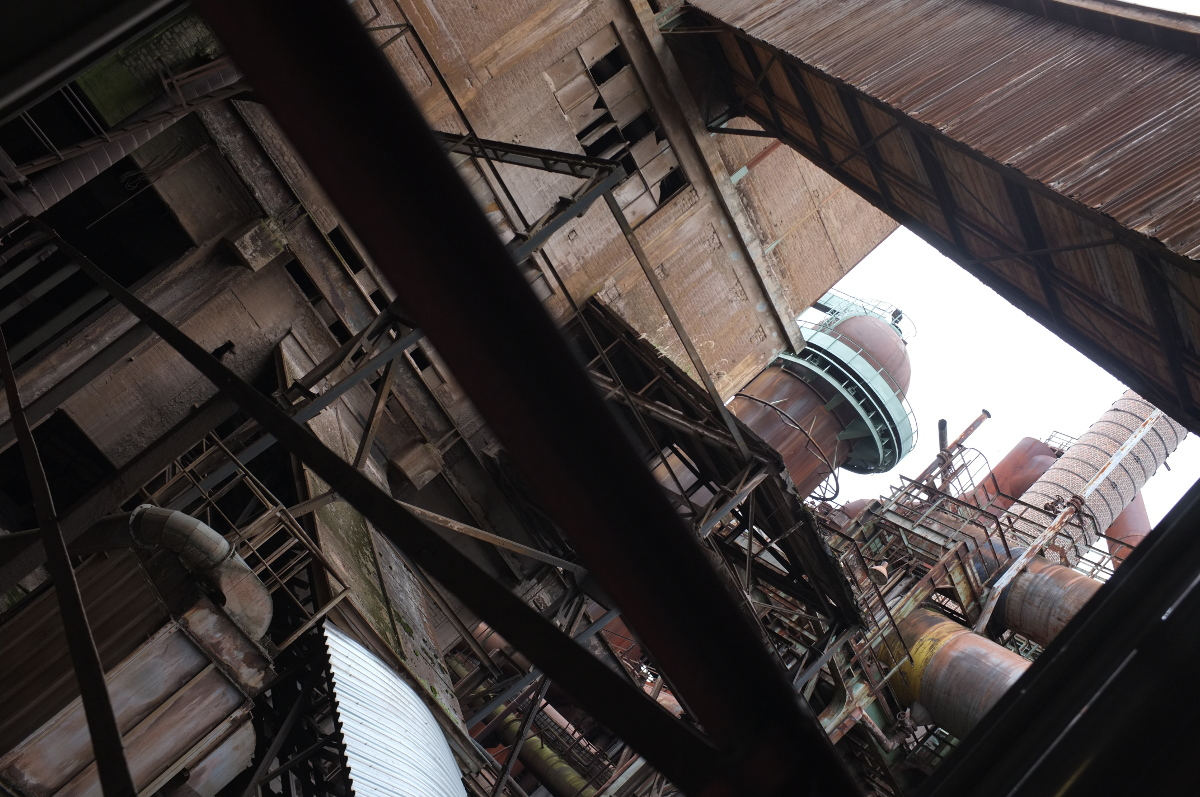
\includegraphics[width=0.4\textwidth]{Examples/example_5.jpg}
  \caption{Völklinger Hütte, *.jpg}
  \label{fig:Huette2}
\end{wrapfigure}
\blindtext


\subsection{Subfigures}
Es ist ebenso möglich, mehrere Abbildungen nebeneinander zu setzen, wie in Abbildung~\ref{fig:Beide} zu sehen ist. Eine separate Referenzierung ist auch möglich: Abbildung~\ref{subfig:abbone}.
\begin{figure}[bth]
  \subfloat[Erstes ...]{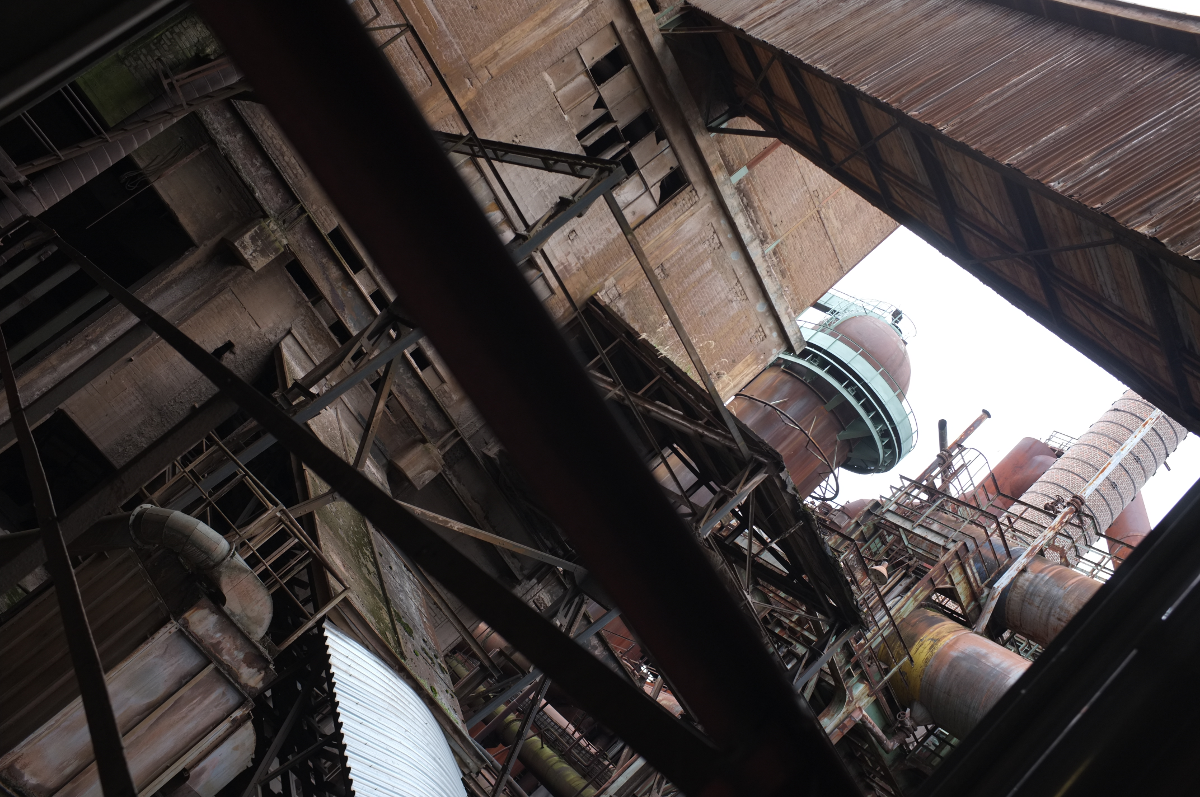
\includegraphics[width=0.49\textwidth]{Examples/example_5.png}\label{subfig:abbone}}\hfill
  \subfloat[... und zweites Bild]{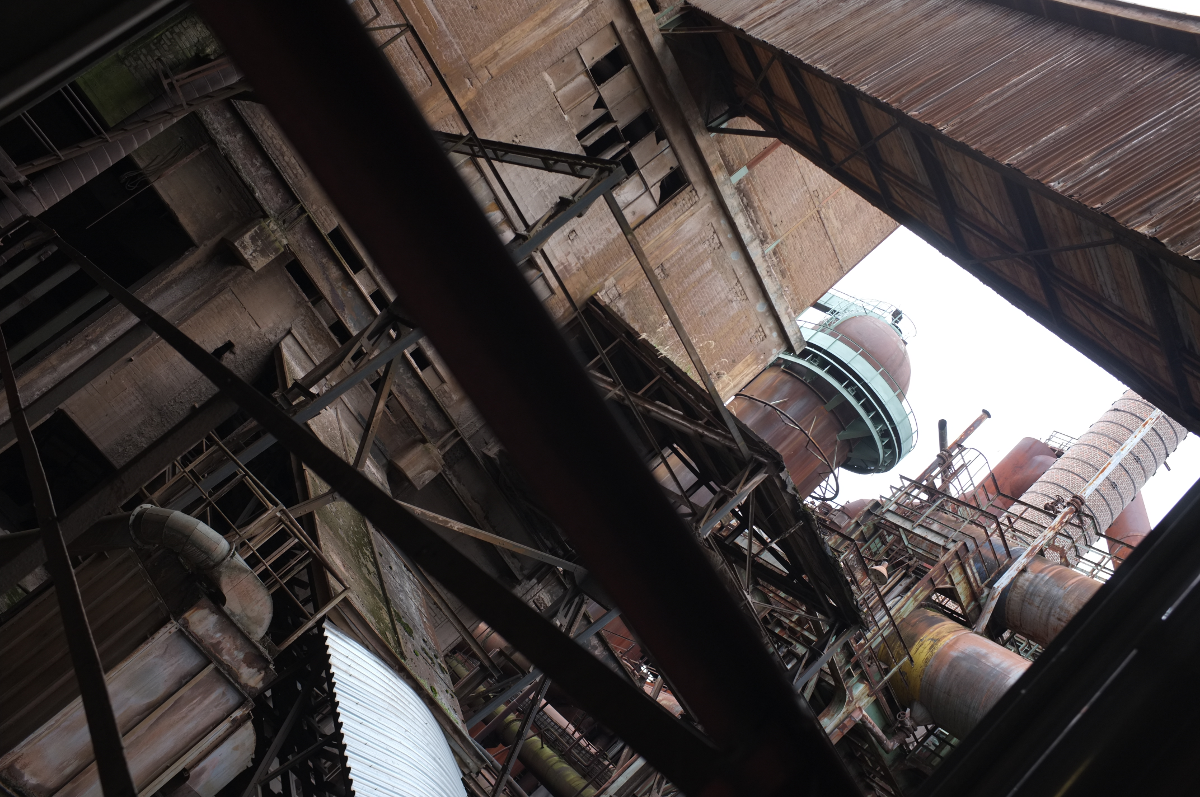
\includegraphics[width=0.49\textwidth]{Examples/example_5.png}\label{subfig:abbtwo}}
  \caption{Mehrere Abbildungen nebeneinander}
  \label{fig:Beide}
\end{figure}


\subsection{Qualitätsunterschiede}
\begin{figure}[p]
	\centering
  \subfloat[\textit{PDF}-Format]{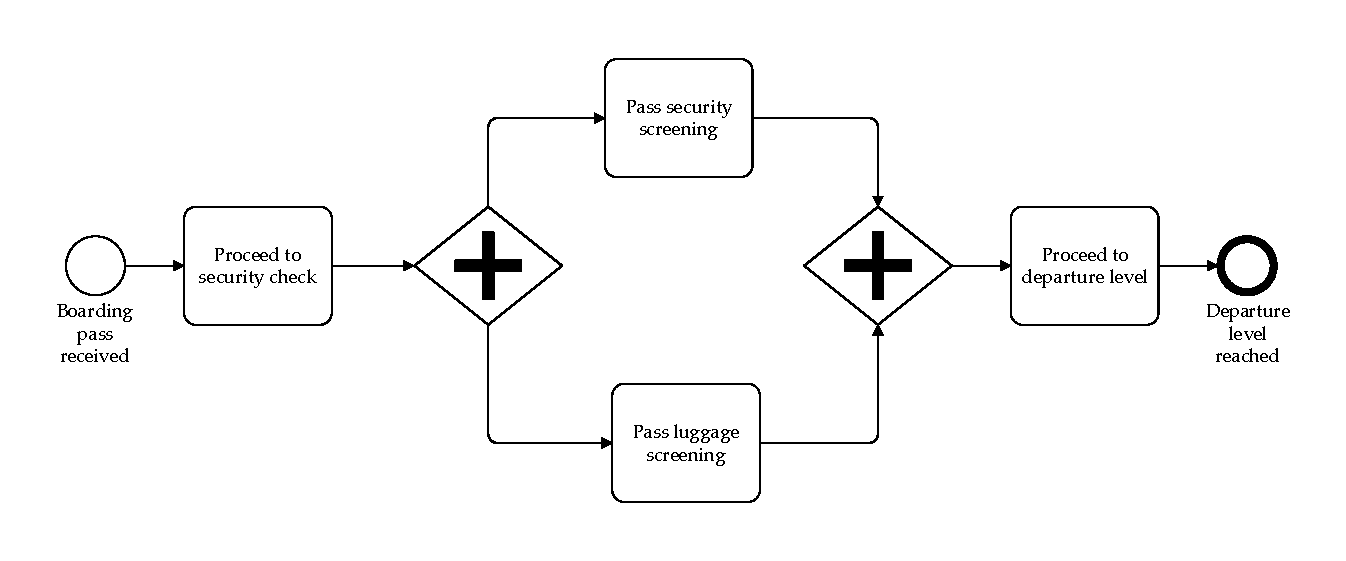
\includegraphics[width=0.65\textwidth]{Examples/bpmn.pdf}} \\
  \subfloat[\textit{JPG}-Format]{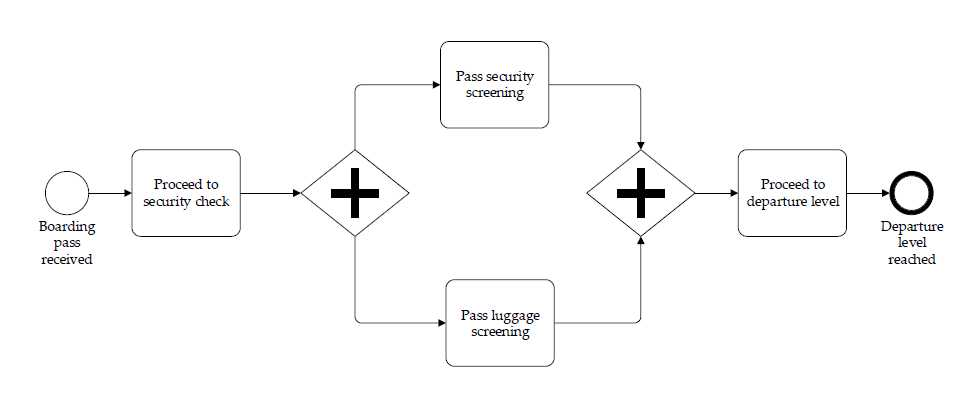
\includegraphics[width=0.65\textwidth]{Examples/bpmn.jpg}}
  \caption{Beide Formate im Vergleich}
  \label{fig:pdfvsjpg}
\end{figure}

\begin{figure}[p]
	\centering
  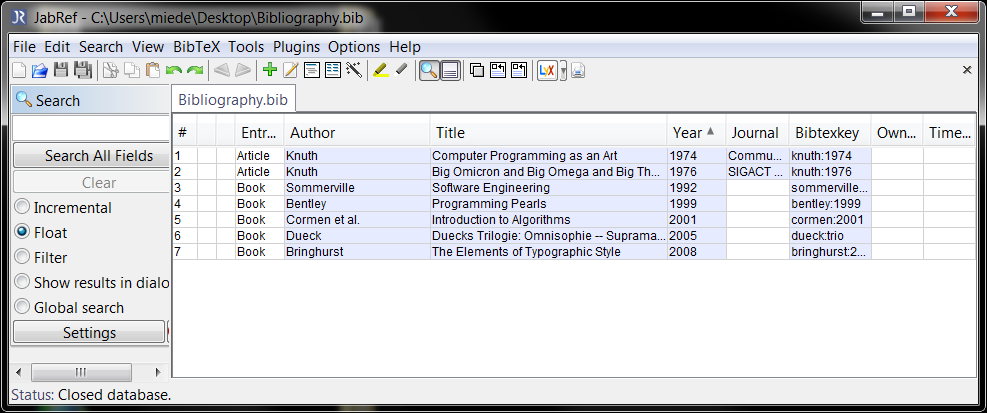
\includegraphics[width=0.65\textwidth]{Examples/jabref.png}
   \caption{\textit{PNG}-Format}
  \label{fig:pngvsjpg1}
\end{figure}

\begin{figure}[p]
	\centering
  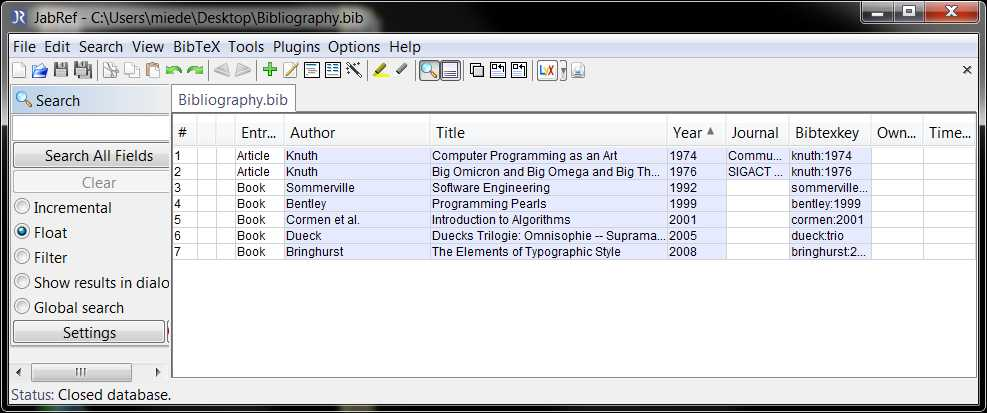
\includegraphics[width=0.65\textwidth]{Examples/jabref.jpg}
   \caption{\textit{JPG}-Format}
  \label{fig:pngvsjpg2}
\end{figure}

Leider haben die unterschiedlichen Grafikformate bedingt durch die unterschiedlichen Kompressionsverfahren einige Schwächen, insbesondere die Umwandlung in das \textit{JPG}-Format erzeugt unangenehme Artefakte im Bild. \autoref{fig:pdfvsjpg} zeigt die Unterschiede zwischen \textit{PDF-Format} und \textit{JPG-Format} im Vergleich. 

Wenn eine \textit{*.pdf}-Datei nicht infrage kommt, beispielsweise bei Screenshots, ist unbedingt das \textit{PNG-Format} vorzuziehen. 
Den Unterschied machen \autoref{fig:pngvsjpg1} und \autoref{fig:pngvsjpg2} deutlich.

\glqq Faustregeln\grqq im Umgang mit Abbildungen:
\begin{itemize}
	\item Diagramme bzw. alles, was Linien usw. enthält: \textit{PDF} (im Vektorformat).
	\item Screenshots bzw. alles, was größere gleichfarbige Flächen enthält: \textit{PNG}.
	\item Der Rest (in der Regel Fotos): \textit{JPEG}.
\end{itemize}





%*******************************
% 			Listings 		   *
%*******************************

\section{Quellcode einbinden}
Das Package \textit{lstlisting} ermöglicht es, Quellcode ansprechend in das Dokument einzubinden. Man kann Quellcode einzeilig einbinden 
mittels \lstinline{\lstinline|Quellcode|}. Dabei ist darauf zu achten, dass der Befehl einmal mit \{ \} und einmal mit | | aufgerufen werden kann, je nachdem, 
welche Zeichen im angegebenen Quelltext genutzt werden. 
Es ist auch möglich eine eigene Umgebung für Quelltext zu schaffen:

\begin{lstlisting}[caption=Erstes Listing,style=Java]
private Umgebung(int i, int k)
{
	System.out.println("Eine Funktion mit " + i + "und" + k ".");
}
\end{lstlisting}  

Wer Quelltext aus externen Dateien einbinden möchte, geht wie folgt vor:

\lstinputlisting
[caption={Externer Quellcode},style=Java]
{Examples/Code.java}

Wie genau der Quellcode formatiert und gefärbt ist, ist in \textit{htwsaar.i.mst.config.tex} hinterlegt, wobei fü verschiedene Sprachen auch eigene Styles angelegt werden
können (hier z.B. für Java).
\section{Mathematische Ausdrücke}
Mathematische Ausdrücke sind eine kleine Kunst für sich. Am allereinfachsten kann man eine Formel, wie \(a + b = c\) in den Fließtext einbinden, wobei LaTeX die Höhe der Ausdrücke der Zeile anpasst,
wie hier zu sehen \(\sum_{y=0}^{x} a\) . In einer Umgebung sieht das schon anders aus:
\begin{equation}
  \sum_{y=0}^{x} a
\end{equation}

Griechische Buchstaben:
\begin{equation}
	\alpha\beta\gamma\delta\epsilon\varepsilon\zeta\eta
	\theta\iota\kappa\lambda\mu\nu\xi\pi\varpi\rho\varrho
	\sigma\tau\upsilon\phi\varphi\chi\psi\omega
\end{equation}

Brüche:
\begin{equation}
	Ergebnis = \frac{a}{b}
\end{equation}

\begin{equation}
	\frac{\sin{\alpha}^2 + \cos{\alpha}^2}{1} = 1
\end{equation}

\begin{equation}
	\frac{-9x}{\frac{2y}{3z+2}}
\end{equation}

Text innerhalb von Formeln:
\begin{equation}
\sum_{y=1}^{n} y = \frac{n*(n+1)}{2}
\quad
\text{Gaußsche Summenformel}
\end{equation}

Hoch- bzw. Tiefstellungen:
\begin{equation}
	x_{i,j}^2
\end{equation}

\begin{equation}
	{x_{i,j}}^2
\end{equation}

\begin{equation}
	x_{n_0}
\end{equation}


Matrizen:
Matrizen werden innerhalb der mathematischen Umgebung als wiederum neue Umgebung eingebunden. Wie bei Tabellen auch werden Zeilen durch \lstinline{\\} und Spalten durch \lstinline{&} getrennt.

\begin{equation}
	\begin{pmatrix} 
		a&b\\
		c&d 
	\end{pmatrix}
\end{equation} 

\begin{equation}
	\begin{vmatrix} 
		a&b\\
		c&d 
	\end{vmatrix}
\end{equation} 

Fallunterscheidung:
\begin{equation}
	f(x) = 
	\begin{cases}
		0, &\text{falls } x < 0 \\
		1, &\text{falls } x \geq 0
	\end{cases}
\end{equation}




%############################################################
\clearpage\section{To-Do-Notes}
Um bei einer längeren Arbeit nicht den Überblick zu verlieren, an welcher Stelle es nötig ist
weiter zu arbeiten, bietet es sich an, kleine Notizen einzufügen. Das Package \textit{todonotes}
stellt eine elegante Lösung bereit, um differenziert und vielfarbig jene Abschnitte zu kennzeichnen,
die einer weiteren Bearbeitung bedürfen.

\subsection*{Beispiel für To-Do-Notes}
Dies hier ist ein Blindtext zum Testen von Textausgaben. Wer diesen Text liest, ist selbst
\todo{Plain todonotes.} schuld. Der Text gibt lediglich den Grauwert der Schrift an. Ist das wirklich so? Ist es
gleichgültig, ob ich schreibe: Dies ist ein Blindtext? oder Huardest gefburn? Kjift?
mitnichten! Ein Blindtext bietet mir wichtige Informationen. An ihm messe ich die Les-
barkeit einer Schrift, ihre Anmutung, \todo{Plain todonotes.}wie harmonisch die Figuren zueinander stehen
und prüfe, wie breit oder schmal sie läuft. Ein Blindtext sollte möglichst viele verschie-
dene Buchstaben enthalten und in der Originalsprache gesetzt sein. Er muss keinen
Sinn ergeben, sollte aber lesbar sein.\todo[nolist]{Todonote that is only shown in the margin and not in
the list of todos.}%
Fremdsprachige Texte wie Lorem ipsum dienen
nicht dem eigentlichen Zweck, da sie eine falsche Anmutung vermitteln. Dies hier ist
ein Blindtext zum Testen von Textausgaben. Wer diesen Text liest, ist selbst schuld. 

\todo[inline]{A very long todonote that certainly will fill more
than a single line in the list of todos. Just to make sure let's add
some more text \ldots}

Der Text gibt lediglich den Grauwert der Schrift an. Ist das wirklich so? Ist es gleichgültig,
ob ich schreibe: Dies ist ein Blindtext? oder Huardest gefburn? Kjift? mitnichten!
\todo[noline]{A note with no line back to the text.}
Ein Blindtext bietet mir wichtige Informationen. An ihm messe ich die Lesbarkeit einer
Schrift, ihre Anmutung, wie harmonisch die Figuren zueinander stehen und prüfe, wie
\todo[caption={A short entry in the list of todos}]{A very long
todonote that certainly will fill more than a single line in the
list of todos \ldots}
breit oder schmal sie läuft. Ein Blindtext sollte möglichst viele verschiedene Buchstaben
enthalten und in der Originalsprache gesetzt sein. Er muss keinen Sinn ergeben, sollte
aber lesbar sein. Fremdsprachige Texte wie Lorem ipsum dienen nicht dem eigentlichen Zweck, 
da sie eine falsche Anmutung vermitteln.
\missingfigure{A figure I have to make \ldots}

%Nummerierte ToDo-Notes
\todox{Erste Nummer...}
\todox{Zweite Nummer...}

%Alles To-Dos als Liste ausgegeben
Nachfolgend wird noch eine Liste aller To-Dos auf einer separaten 
Seite ausgegeben.
%\begingroup
	%\let\clearpage\relax
	%\let\cleardoublepage\relax
	\listoftodos
%\endgroup 


 Abschlussarbeit geht!
%\cleardoublepage\include{Chapters/KapitelBachelorarbeit} % <<< Hier alle Chapter der Abschlussarbeit (einzeln) einbinden

%********************************************************************
% Bibliography/References
%*******************************************************
\cleardoublepage%********************************************************************
% Bibliography
%*******************************************************
\printbibliography

%********************************************************************
% List of Figures etc.
%*******************************************************
\cleardoublepage%*******************************************************
% Verzeichnisse (Abbildungen, Tabellen, Listings, etc.)
%*******************************************************
\cleardoublepage
\begingroup
	\let\clearpage\relax
	\let\cleardoublepage\relax
	\listoffigures
	\listoftables
	%\addcontentsline{toc}{chapter}{\lstlistlistingname}
	\lstlistoflistings 
\endgroup 
%*******************************************************
% Abkürzungsverzeichnis
%*******************************************************
\chapter*{Abkürzungsverzeichnis}
\addcontentsline{toc}{chapter}{Abkürzungsverzeichnis}	
	%Hier alle benötigten Abkürzungen einfügen
	\begin{acronym}[WLAN] % LONGEST ACRONYM HERE FOR CORRECT SPACING
	    \acro{WLAN}{Wireless Local Area Network}
	    \acro{TCP}{Transmission Control Protocol}
	    \acro{GoF}{Gang of Four}
	\end{acronym}
	
	

% ********************************************************************
% Appendix/Anhang
%***************************************************************
%\appendix
%\part*{Anhang}
%\cleardoublepage%********************************************************************
% Appendix
%*******************************************************
\chapter{Erster Abschnitt des Anhangs}
\section*{Weitere 8192 Bit Primzahlen} 
1. Primzahl: \\
164448 180681 332856 932919 221079 406875 222245 392841 097816 487396 445158 622479 499799 434642 647441 405685 104617 865576 724909 860296 931750 129737 767216 694383 619789 025341 452240 959026 117432 528709 543618 224156 295506 958642 510160 814938 273358 619516 779384 170673 413680 182305 838032 148369 021449 473709 603650 212890 289715 456945 042625 495388 261136 358474 815184 086400 157910 220345 573541 434405 842267 628330 533110 631980 035825 544962 065625 468992 305435 553683 877572 152876 077964 115502 824760 593862 714937 988061 337941 253343 964870 798124 056398 641971 602856 386168 741346 850204 419477 893561 282419 626159 955911 411956 570848 870505 110320 227207 339694 484182 877002 074704 175122 335331 312606 597549 997437 019159 011395 275947 865958 515180 597427 819417 068307 454735 386255 831798 798609 472760 579747 003970 997332 748314 872387 146222 066028 569353 408289 510366 836644 203558 100663 550138 227170 003542 324779 783323 180274 479100 627563 087777 643761 026894 258555 157167 413497 765679 861741 302521 360965 468998 343773 389722 583751 204323 145122 802605 561626 145423 798698 884461 284280 788800 939176 373345 946938 101644 910966 929924 002096 767111 042625 469154 433847 319465 703014 786490 409151 817076 669197 668892 294188 629132 220264 676510 130862 384779 839199 821590 182277 977417 940145 107673 030037 607401 625779 633199 211952 655853 383847 855863 131001 045017 972863 223339 419951 110289 905418 068855 123866 694988 146597 988891 553792 298990 955916 002493 419799 458688 639661 862912 616104 628874 927134 414440 062885 263803 685352 616723 045058 988271 795195 849619 627384 092709 108711 490147 755056 352581 600388 037234 634022 313629 615436 679568 668056 496796 699324 397356 717240 524335 930325 619569 512662 992006 056652 291352 928185 912962 826364 219522 002546 559814 194597 218969 747944 884174 920287 554023 254511 854741 066723 443796 550870 509238 493888 852196 562823 272836 938807 446407 697003 046228 135406 311918 274933 079219 544177 621010 600739 852732 928807 119314 857520 983872 304165 488365 547217 305388 957367 872905 359424 400919 139588 696785 590452 962142 452382 131788 928822 646256 767824 519943 584772 372342 595356 646238 793599 250744 824827 366650 534015 787661 046447 120717 830558 132037 372400 454202 729586 606491 799122 560862 313867 425098 111591 832164 777324 726954 620173 289643 120454 190278 656548 627915 316093 641943 940898 015263 973528 075981 007959 360241 383512 113351 661621 802751 365887 042466 319078 007567 865685 264410 068999 888707 589689 573399 376701 377471 716243 880538 784151 146367 551112 637166 614547 586791 656341 560552 153345 253665 070314 393525 974077 775677 626353 513030 548667 651308 390415 341268 000350 326795 644132 727210 691916 369934 056251 384172 259608 250030 950882 336941 367837 571527 130371 594781 156722 562416 295329
\newpage
2.Primzahl:\\
138102 547630 171315 997311 901730 542075 110921 280360 005926 068554 750588 340316 176608 045812 226378 223623 206844 863335 021549 839943 626379 580028 596582 919776 908841 025590 525516 173388 536925 007792 993850 508668 686242 651389 477532 581530 325008 490392 305046 787095 469021 265839 427530 502911 410468 490981 033935 199149 748308 553815 251661 690898 268888 774136 564193 886417 843252 401253 633904 224405 927165 677934 723377 252428 042713 446073 316254 066634 554789 364308 182167 721614 312804 669613 192533 031712 318368 089080 171752 323622 863822 928893 013429 621584 548427 170224 384080 400521 868234 307831 635853 310005 581422 043269 320001 278963 547161 423571 817292 798160 277501 706620 618970 751449 650401 682633 635089 262981 448000 391248 684592 525578 166810 338133 135598 605548 763001 362426 253246 719067 066405 373823 256514 297533 870920 989594 361362 614904 898246 107309 144633 513072 556772 323987 566048 674725 278486 849504 427244 748292 610444 623941 636547 193676 303946 914491 666033 729595 167273 681723 652806 661564 437073 218654 602193 285654 698052 499746 975924 812177 730086 072704 869255 560721 591450 103933 978823 720567 921710 556386 726176 409270 063752 784670 520023 890153 836090 770504 566257 501741 807894 035623 458879 574659 166870 635813 990518 280067 721537 151096 597288 910093 611764 435718 488069 514646 257016 870595 532374 487319 535508 773536 571523 707589 895665 677001 414428 735760 431339 162182 329572 606585 001987 723837 942494 116723 124252 276031 743832 489760 121008 392160 376839 556970 708044 213878 285971 477361 984494 014389 940037 442565 386868 489551 985305 597149 374506 836007 414174 008151 455122 195375 450800 039704 753129 226242 756284 020756 385291 458700 591766 803751 922044 361930 713545 924973 330439 057760 116877 077169 642004 264221 635627 203576 454143 803291 892982 606392 111877 980709 823085 247443 169217 707666 521418 989795 540281 691475 966531 431323 763651 821730 143486 156467 398124 733590 839820 392949 682141 309067 460970 320718 676308 988769 614786 287954 400034 977924 707404 607751 856774 242480 278872 330182 644893 118018 319476 580527 975050 505448 739354 482521 366151 633329 079128 200811 177088 986491 717621 823639 489332 899707 191908 427012 581020 872300 060481 343636 078936 232381 272675 771649 342340 406639 836373 960821 677221 044364 341613 418517 176412 863313 886940 833976 878178 414315 387661 256595 838212 899902 437079 914509 838001 157324 802028 524873 820201 880936 769825 900737 159661 654136 040554 056570 386758 027098 748348 352395 291123 093370 591162 476725 396763 187371 413262 638974 088056 067580 076505 368986 300675 876848 020988 524067 971878 394002 548169 323256 029860 550016 300093 059106 365019 528103 651961 437398 242647 949163 973097 891644 457544 894286 619653 042323 065692 312564 533352 316527 543985 085250 999457
\\
\newpage
3. Primzahl: \\
917365 233753 903939 620457 021505 304714 911813 951619 192279 871010 498329 643482 506013 138900 835998 797450 243336 281697 759424 691961 200626 170113 125151 901910 344027 738974 952143 128345 783067 178864 691160 917446 655861 169150 312302 845253 037651 008551 989797 146233 671915 513406 428906 160835 052621 709702 108202 271446 711123 221622 733917 420979 489209 389592 784030 956061 897699 790523 125997 157073 613039 878485 470797 136586 317013 877365 289590 957562 766118 515152 934790 360987 187459 164789 537675 901848 418658 603970 948020 867494 178036 379115 748972 157694 810451 488508 864816 190126 737574 856918 693546 135213 264445 428296 449358 940480 344453 671989 381582 926370 490148 835469 755795 461550 492756 635480 391722 363251 909312 947601 149658 482365 934742 264967 987261 466145 963647 897490 272042 514351 925643 783662 169811 605129 653492 338162 369388 752251 821697 999804 107614 099675 103929 333572 049319 469736 092002 468465 655371 652031 447356 095625 275574 499128 988759 705337 980638 360086 250695 791151 526433 194248 300373 600271 304358 498195 669382 408521 547137 309724 838439 286732 026832 465579 314728 307048 518117 466953 674003 336481 950505 150397 339302 038980 129610 532109 568864 069386 764292 735848 933740 307257 023048 835362 064933 660985 285985 838227 266534 031062 556507 920510 696776 589913 310291 585861 676953 751461 798475 805412 265844 420904 839962 227557 548294 441445 414230 126172 633123 372425 879636 740746 555124 950266 072193 714328 893400 494364 075668 896534 898785 624919 114457 286257 960159 152313 398898 135640 253264 204095 343830 577350 256806 239430 744920 553825 408510 179639 847260 809163 512620 943119 403661 791634 561114 747349 583234 600800 272243 678352 679489 622599 779819 736754 925849 278110 719165 662739 484435 131244 688938 841883 711162 317771 575095 746869 995988 967126 874255 488414 352997 479582 959527 717304 441450 995711 295010 255507 404197 833781 247689 190910 467790 829373 533107 376653 479787 243737 983436 701642 887284 964321 532191 199950 864478 692672 482409 459006 262951 224390 015616 689073 290666 106850 995927 845135 383652 387494 267076 222316 646579 080823 320744 585640 675051 625876 852933 991219 817944 541002 242711 395928 276025 602306 773509 897013 306405 575656 143175 958224 005122 888457 161972 132762 001418 215250 460390 220986 074979 853299 419092 018563 230882 688553 502857 385036 826258 073342 052156 338927 721621 070447 834758 394573 197678 573209 985712 719431 728246 480028 728775 181092 735247 871973 271805 162281 843082 713528 075116 745351 312902 870730 567228 492777 093115 708351 322503 935015 611574 516762 283278 830527 857764 573507 977290 409447 552836 202748 543311 651449 999136 268317 781344 232257 444300 980076 968669 712405 437615 951790 419410 050792 469269 740593 941674 842368 908280 859579 928297 481982 759497
\\


%*******************************************************
%\cleardoublepage\pagestyle{empty}

\hfill

\vfill


\pdfbookmark[0]{Kolophon}{colophon}
\section*{Kolophon}
Dieses Dokument wurde mit der \LaTeX-Vorlage für Abschlussarbeiten an der htw saar im Bereich Informatik/Mechatronik-Sensortechnik erstellt (\currentVersion). Die Vorlage wurde von Yves Hary und Andr\'e Miede entwickelt (mit freundlicher Unterstützung von Thomas Kretschmer, Helmut G. Folz und Martina Lehser). Daten: (F)\makeatletter\f@size\makeatother\ -- (B)\the\textwidth\ -- (H)\the\textheight\ 


\end{document}
% ********************************************************************
